\documentclass[a4paper,12pt]{article}
\usepackage{graphicx}
\usepackage[a4paper, total={6in, 9in}]{geometry}
\usepackage[T1]{fontenc}
\usepackage[utf8]{inputenc}
\usepackage{graphicx}
\usepackage{tikz}
\usepackage{float}
\usepackage{mathtools}
\usepackage{fancyhdr}
\usepackage{caption}
\usepackage{textgreek}
\usepackage{yfonts}
\usepackage{amssymb}
\usepackage{hyperref}
\usepackage{amsmath}
\usepackage{systeme}
\hypersetup{
    colorlinks=true,
    linkcolor=blue,
    filecolor=magenta,
    urlcolor=cyan,
    pdftitle={Overleaf Example},
    pdfpagemode=FullScreen,
    }

\urlstyle{same}
\let\empty\varnothing
\let\eqv\Longleftrightarrow
\renewcommand{\figurename}{Figura}
\renewcommand{\contentsname}{Índice}
\renewcommand{\refname}{Bibliografia}
\usepackage{longtable}
\pagestyle{fancy}
\date{Março 2022}
\title{ \\ \large {Initial Report}}
\author{João Barreiros C. Rodrigues}

\begin{document}
        \pagenumbering{gobble}
        \begin{titlepage} % Suppresses displaying the page number on the title page and the subsequent page counts as page 1
        	\newcommand{\HRule}{\rule{\linewidth}{0.5mm}} % Defines a new command for horizontal lines, change thickness here
        	\center % Centre everything on the page
        	\textsc{\LARGE Instituto Superior Técnico}\\[1.5cm] % Main heading such as the name of your university/college
        	\textsc{\Large Licenciatura em Engenharia Eletrotécnica e de Computadores}\\[0.25cm]
		\textsc{\Large UC Circuitos Eletrónicos}\\[0.25cm]
        	\HRule\\[0.4cm]
        	{\LARGE\bfseries Relatório Laboratorial}\\[0.4cm] % Title of your document
        	{\huge\bfseries Amplificador com Transístores Bipolares}\\[0.4cm] % Title of your document
        	\HRule\\[1.5cm]
		Gonçalo \textsc{Bernardino Frazão}, nº 99945 \\
        	João \textsc{Barreiros C. Rodrigues}, nº 99968\\
		José \textsc{Lopes}, nº 100001\\ 
        	\vfill\vfill\vfill % Position the date 3/4 down the remaining page
        	{\large Maio 2022} % Date, change the \today to a set date if you want to be precise
        	\vfill % Push the date up 1/4 of the remaining page
	\end{titlepage}
        \pagenumbering{arabic}
        \newpage
        	\tableofcontents
        \clearpage
		\section{Questão 4}
			\subsection{Modelo e Questão 4.1}
				Através da análise nodal e de malha do circuito introduzido no \textit{LTSpice} obtêm-se os seguintes valores:\\
				\begin{minipage}[H]{0.45\textwidth}
				\begin{table}[H]
					\centering
					\begin{tabular}{|l|c|}
						\hline
						\textbf{VB1}  &  1.7457 V\\ \hline
						\textbf{VBE1} &  0.6354 V\\ \hline
						\textbf{VCE1} &  1.9190 V\\ \hline
						\textbf{VO1}  &  3.0293 V\\ \hline
						\textbf{VBE2} &  0.63796 V\\ \hline
						\textbf{VCE2} &  2.6086 V\\ \hline
						\textbf{Ic1}  &  0.89 mA\\ \hline
						\textbf{Ic2}  &  0.99 mA\\ \hline
					\end{tabular}
				\end{table}

				\end{minipage}
				\hfill
				\begin{minipage}[H]{0.45\textwidth}
                                          \centering
                                          \captionsetup{justification=centering}
                                          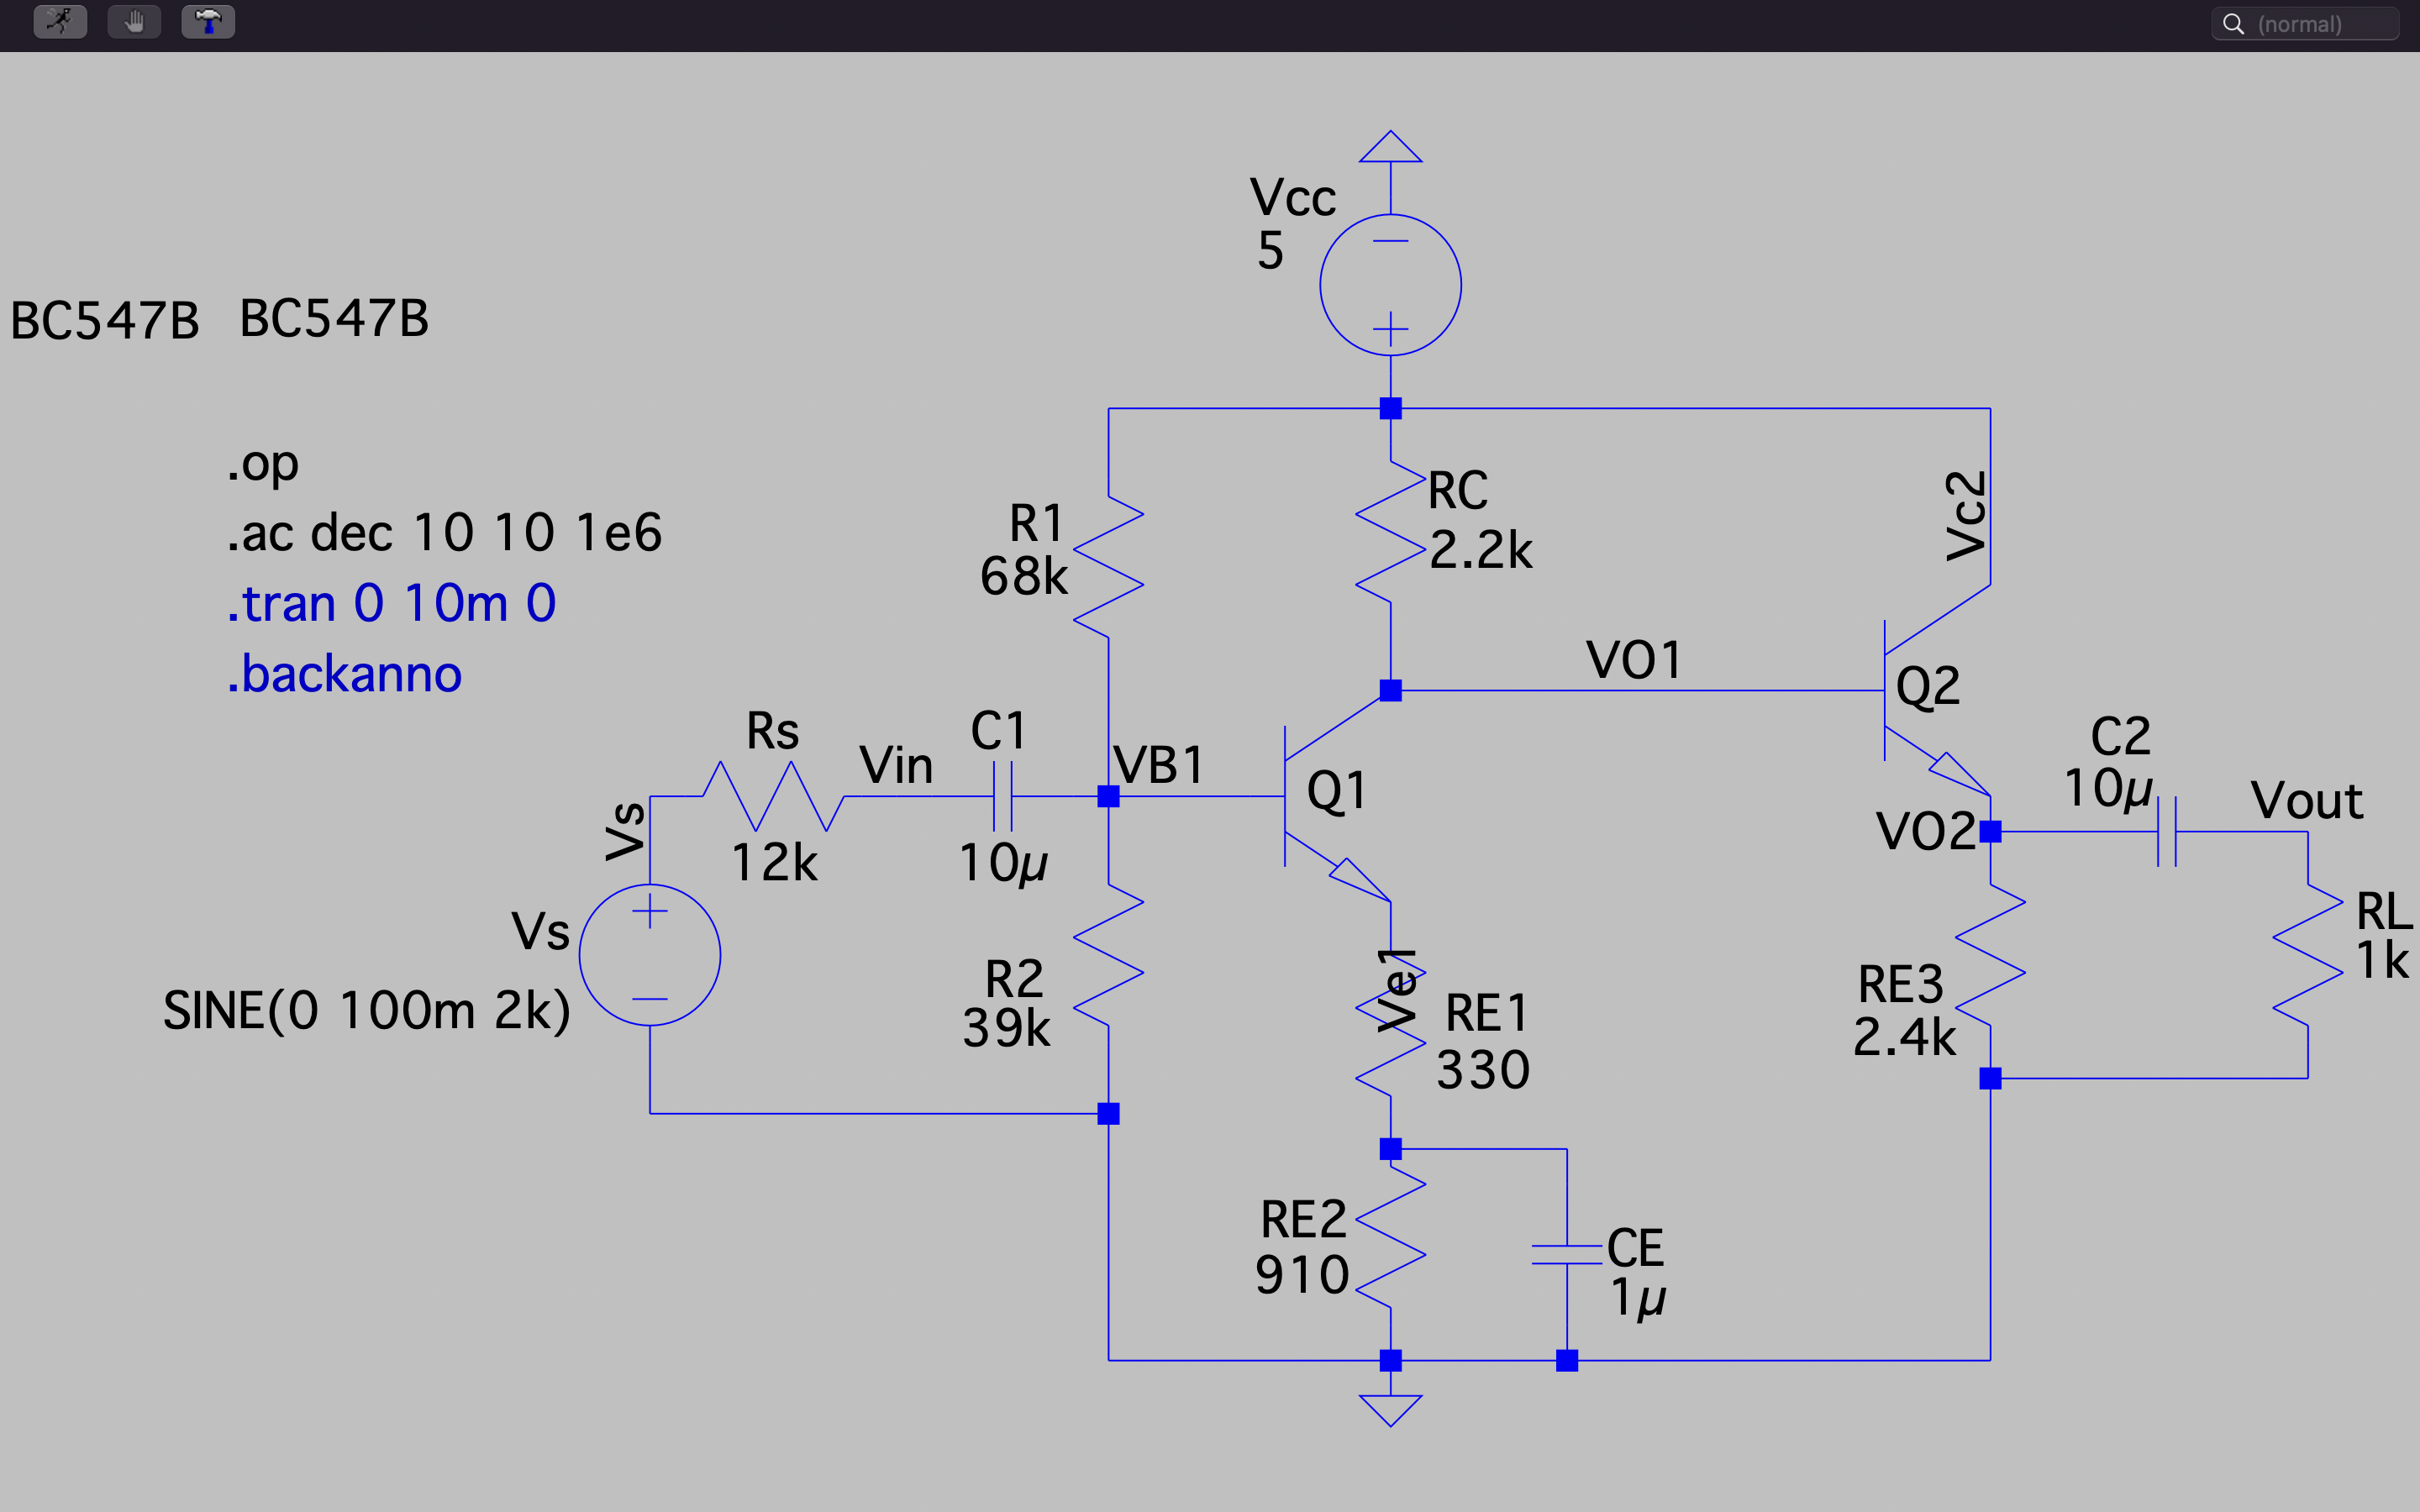
\includegraphics[scale=0.15\textscale]{spice.png}
                                        \captionof{figure}{Simulação do amplificador de dois andares, com transístores BJT, BC547B.}
                                  
				\end{minipage}

				

			\subsection{Questão 4.2}
				\begin{figure}[H]
    					\centering
					\captionsetup{justification=centering}
    					\begin{minipage}[t]{0.45\textwidth}
        					\centering
					        					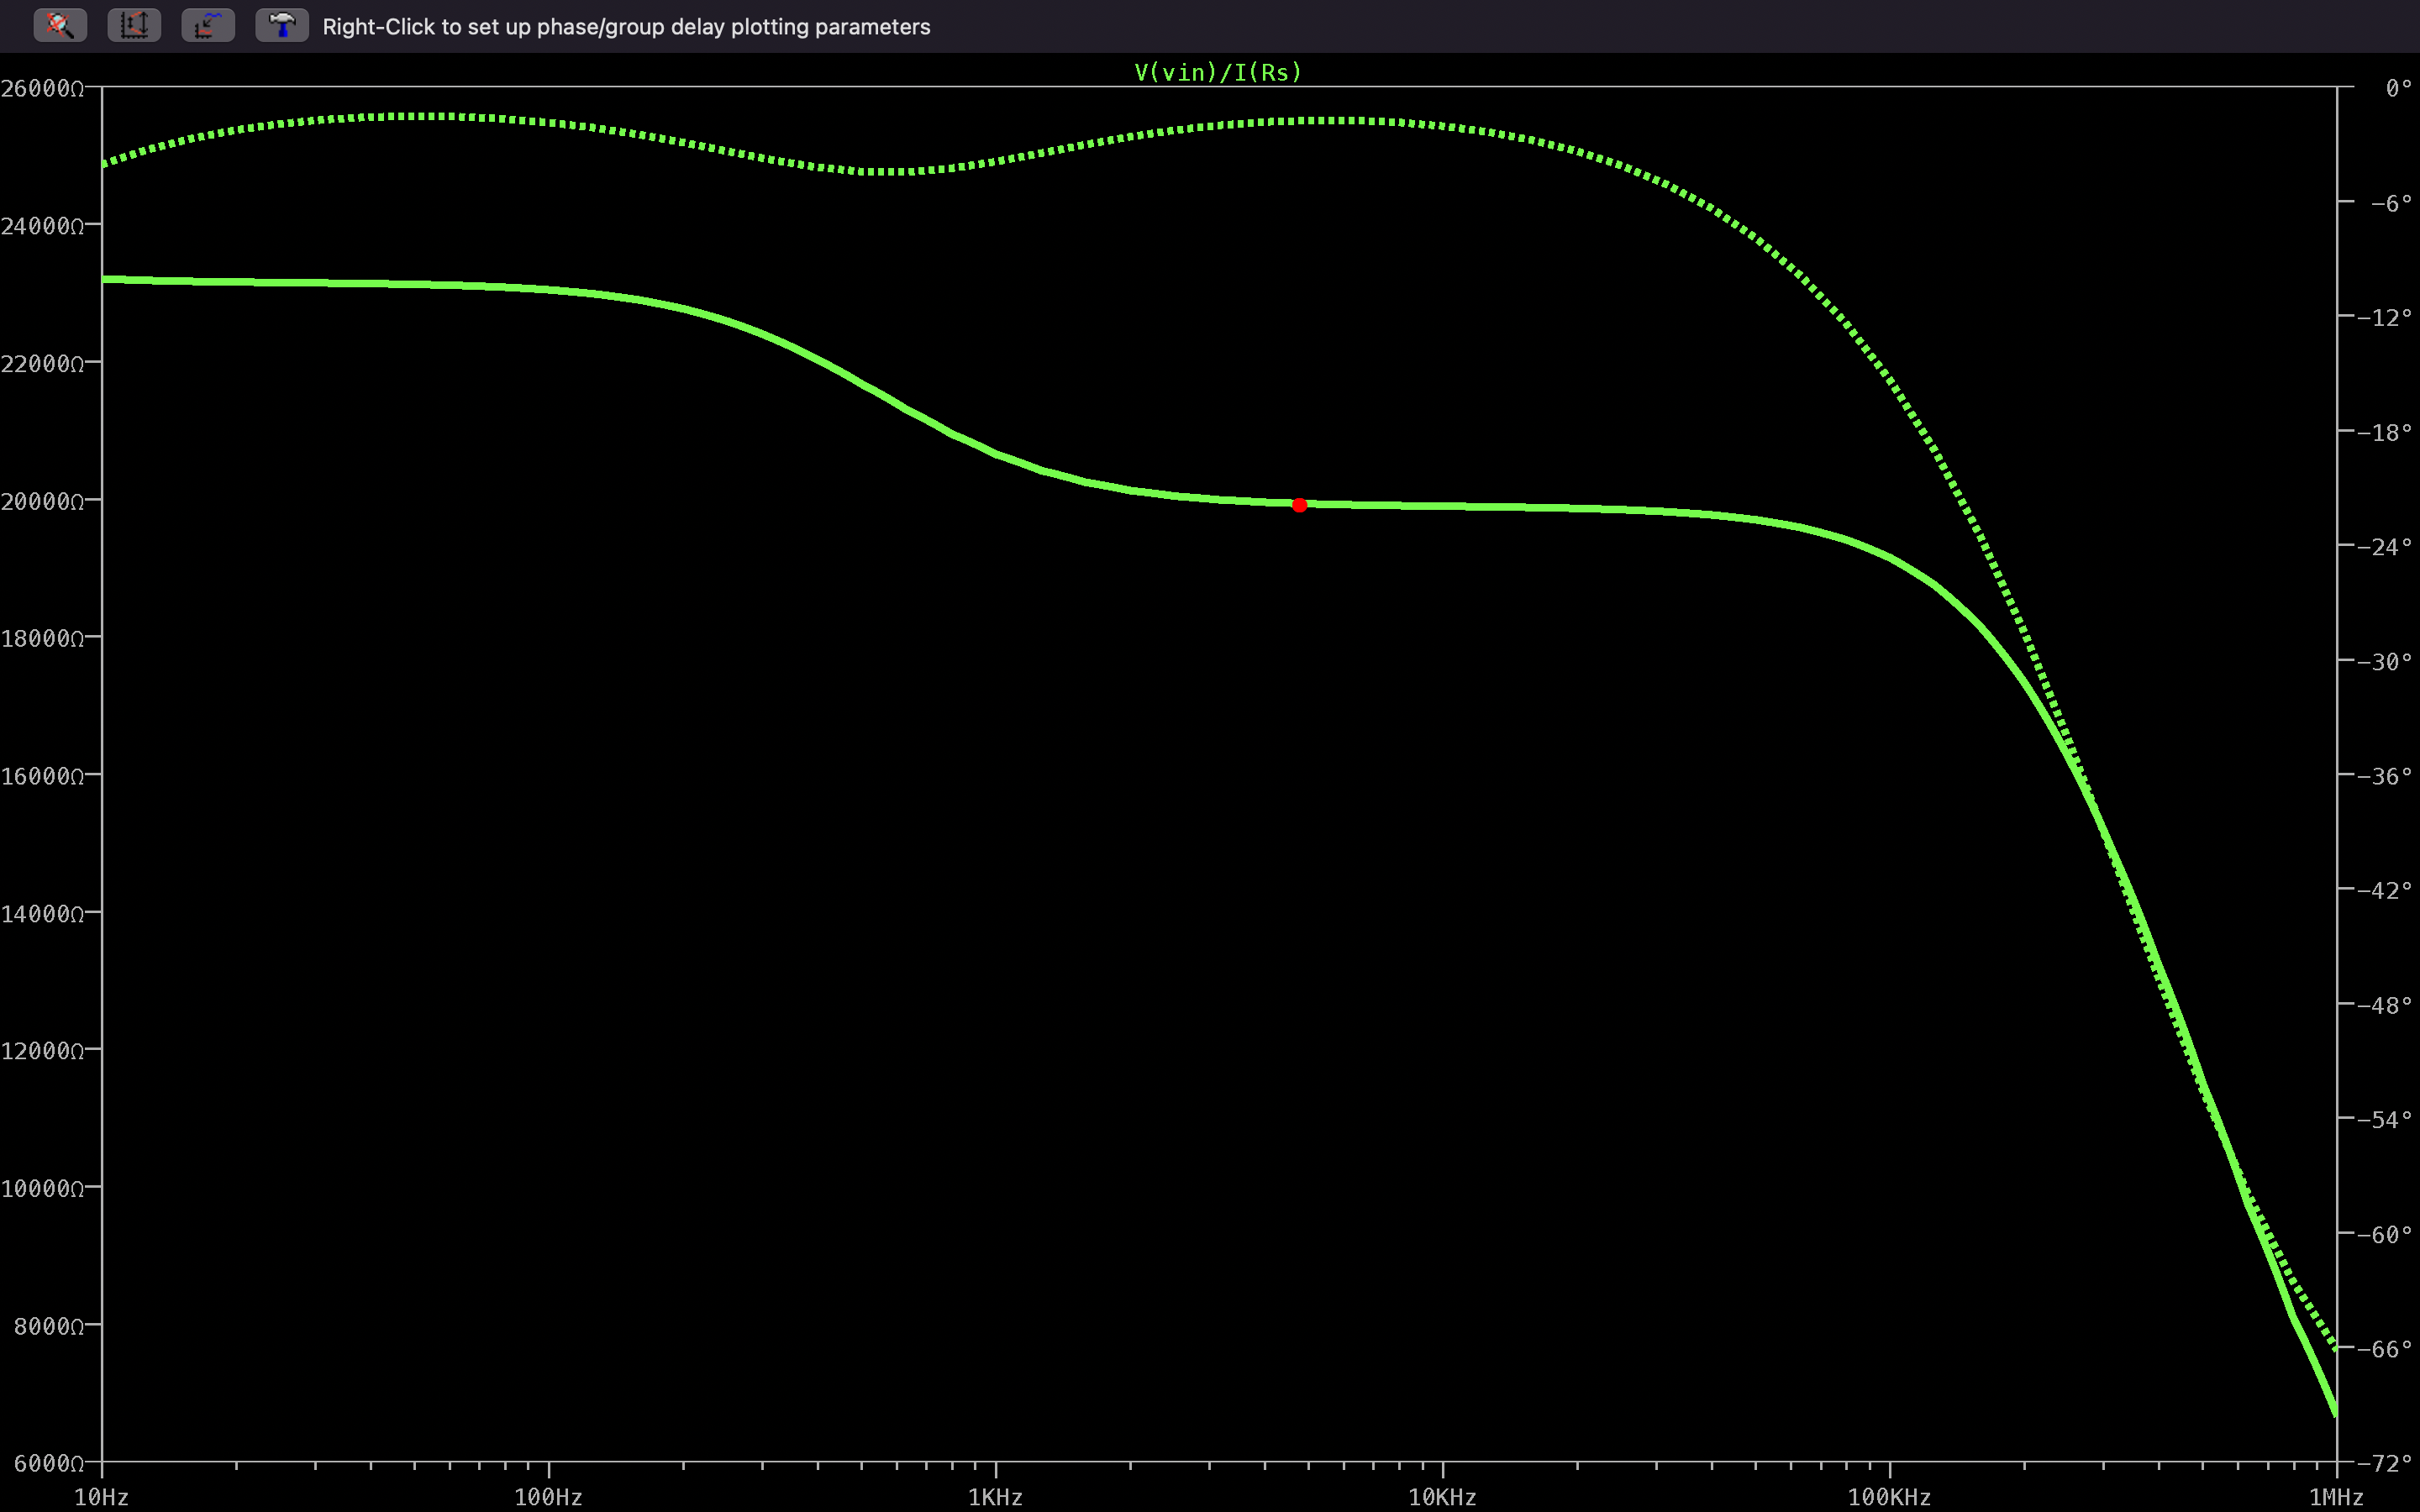
\includegraphics[width=1.2\textwidth]{4.2-1.png} % first figure itself
        					\caption{Impedância R$_{I1}$ em função da frequência de entrada, obtida através do quociente entre valores simulados V$_{B1}$ e Ib$_{Q1}$. A vermelho a Impedância R$_{I1}$(5KHz)=19.9 k\Omega}
    					\end{minipage}\hfill
    					\begin{minipage}[t]{0.45\textwidth}
        					\centering
						
        					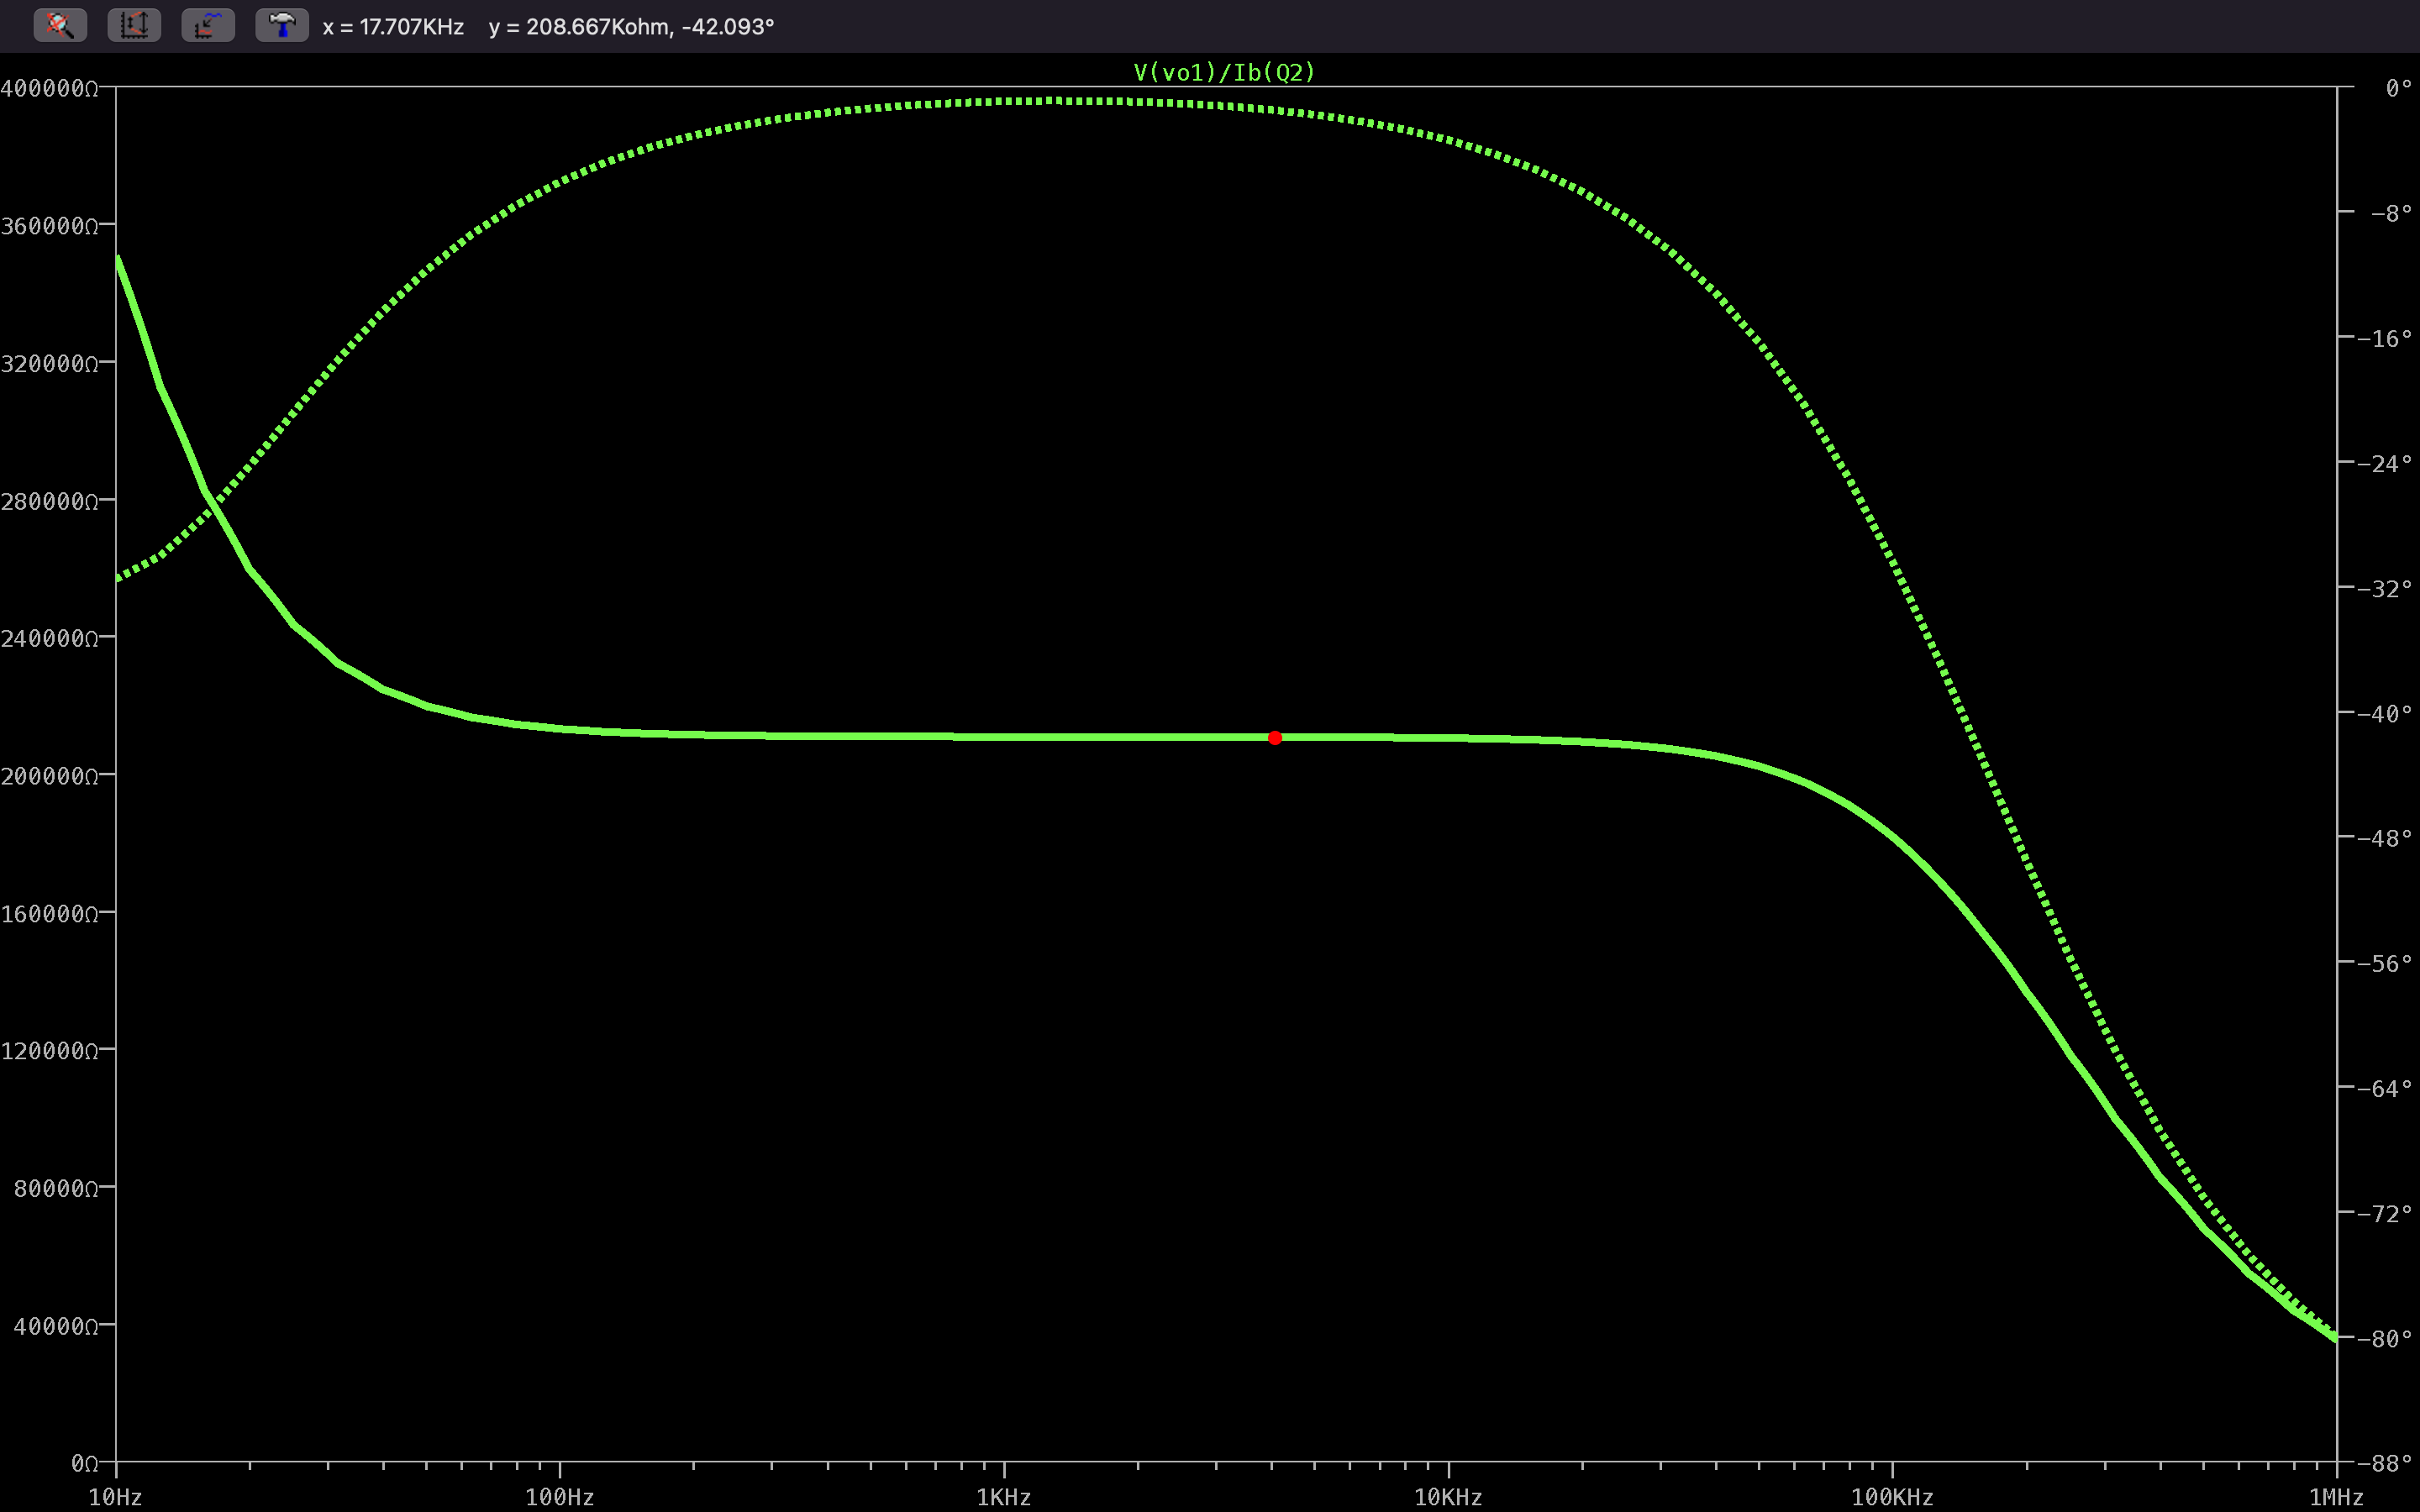
\includegraphics[width=1.2\textwidth]{4.2-2.png} % second figure itself
        					\caption{Impedância R$_{I1}$ em função da frequência de entrada, obtida através do quociente entre valores simulados V$_{B2}$ e Ib$_{Q2}$. A vermelho a Impedância R$_{I2}$(5KHz)=210 k\Omega}
    						\end{minipage}
				\end{figure}

			\subsection{Questão 4.3}
				\begin{figure}[H]
    					\centering
    					\begin{minipage}{0.45\textwidth}
        					\centering
        					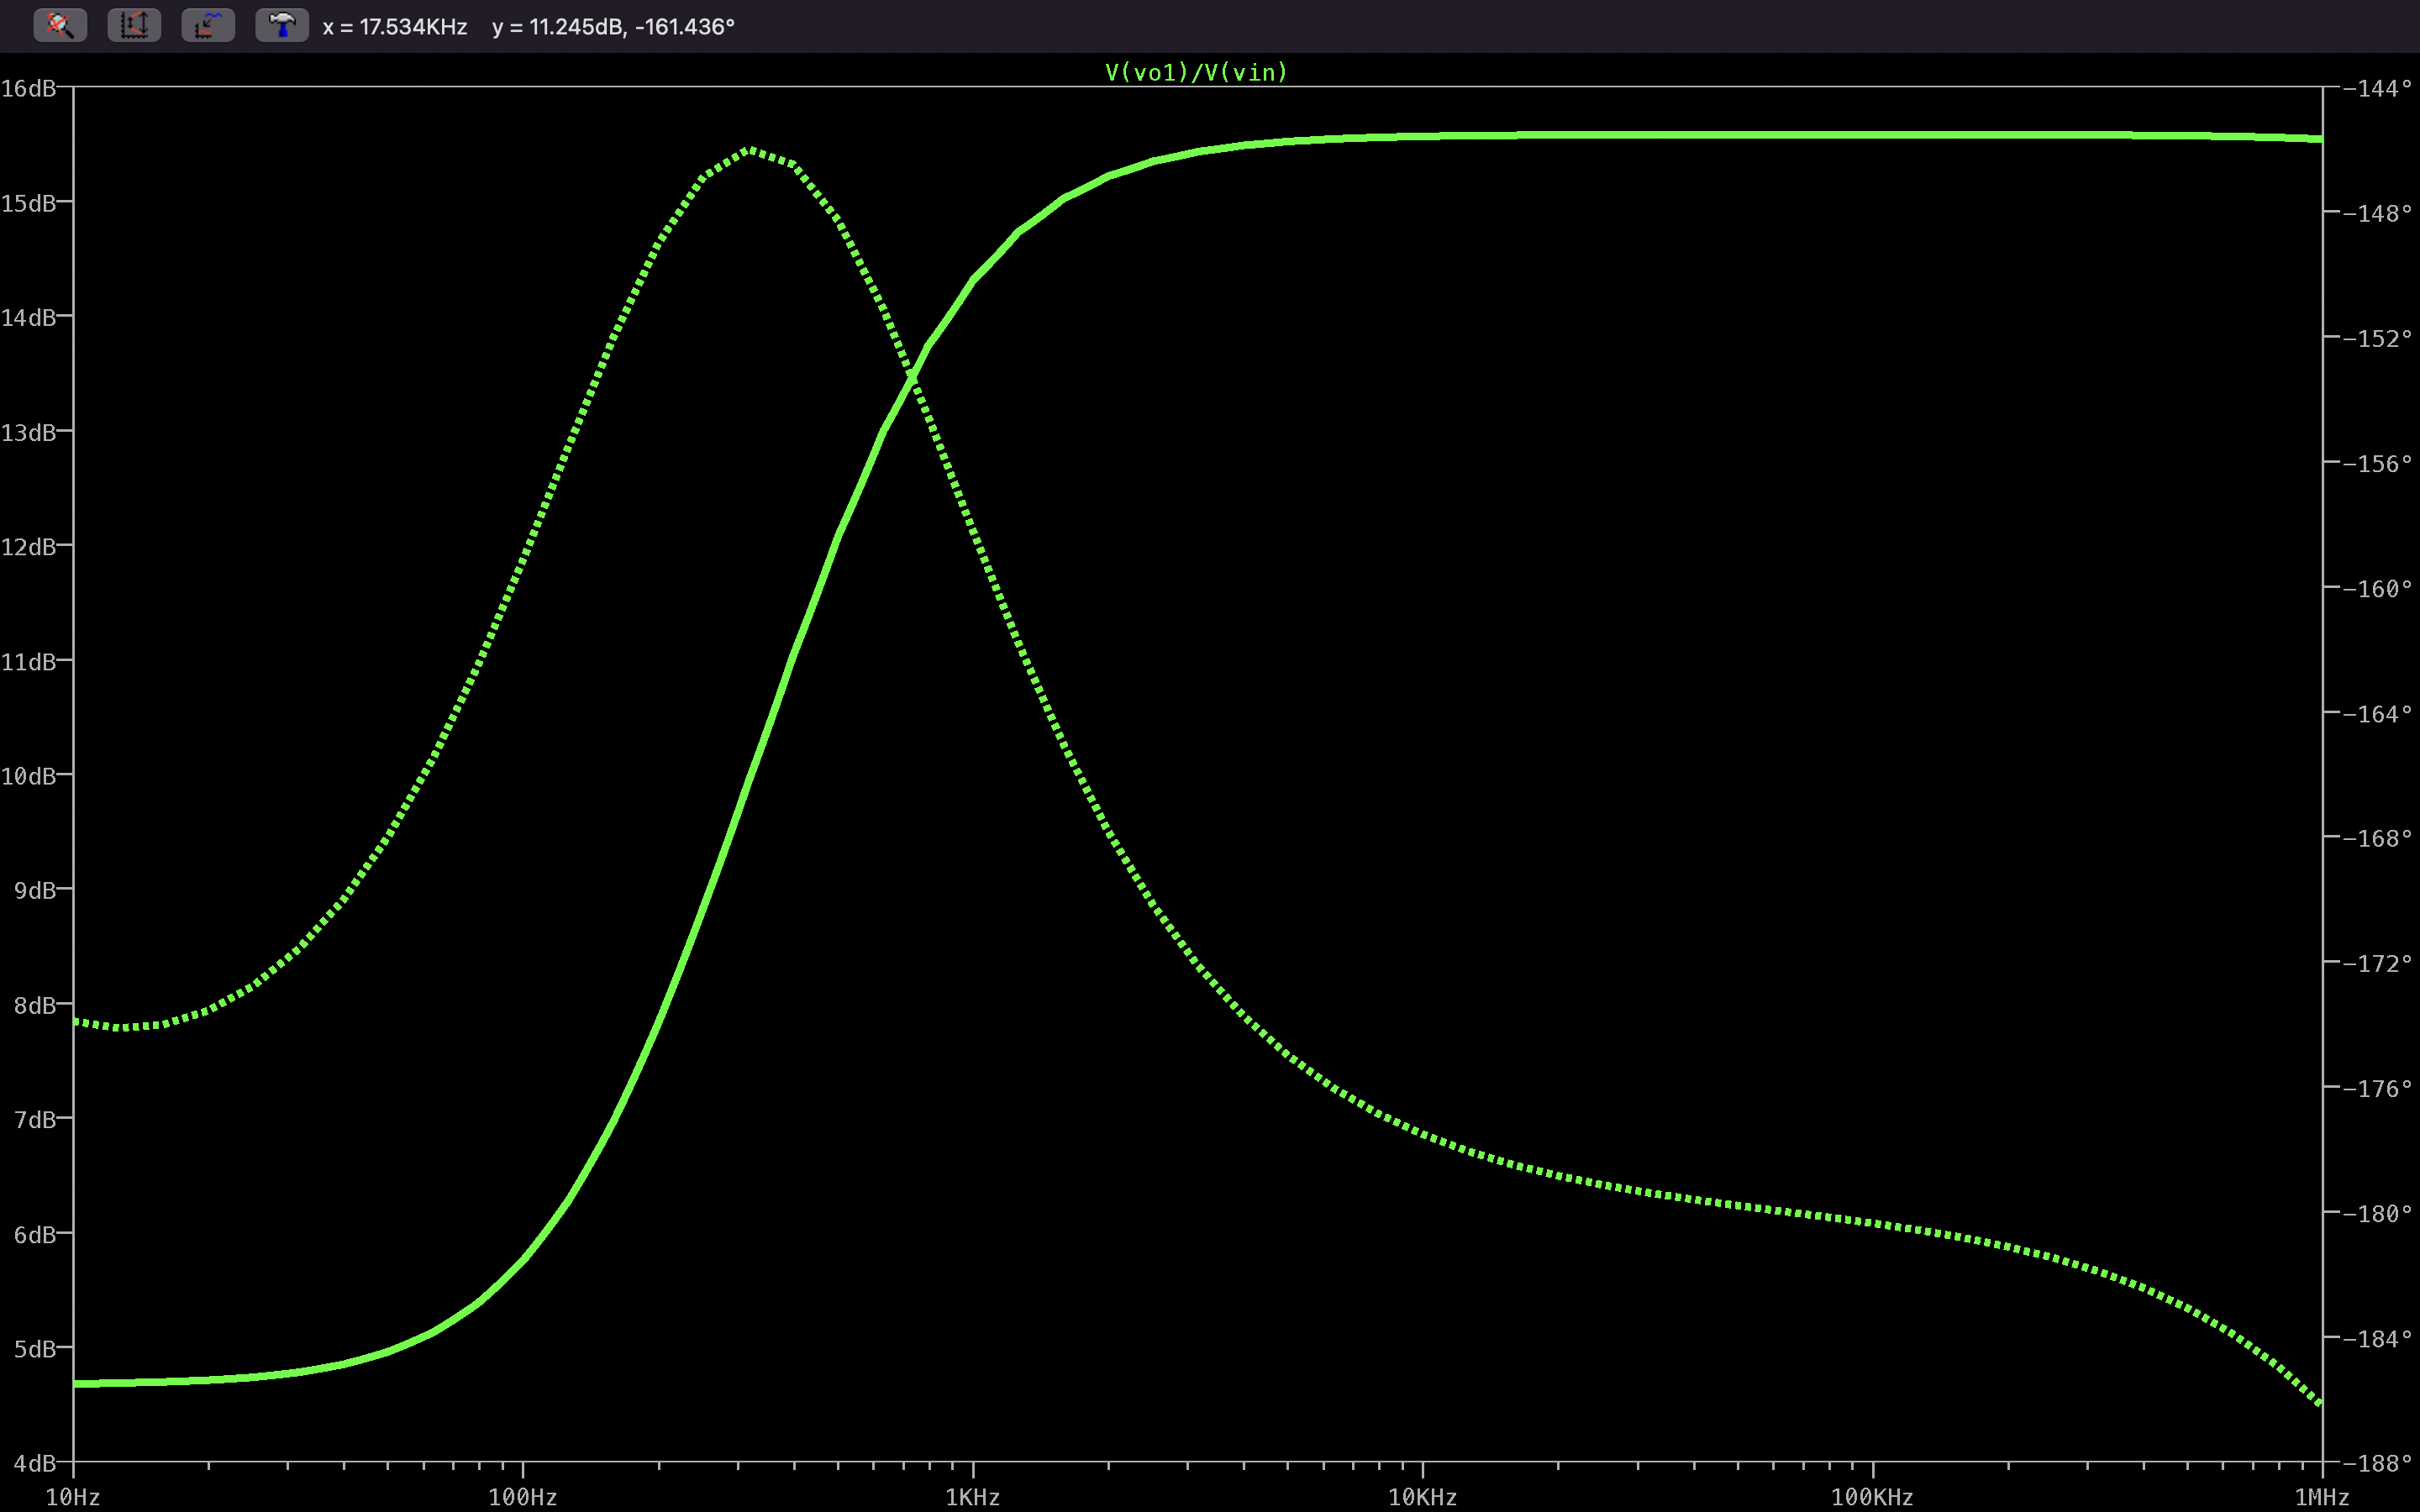
\includegraphics[width=0.9\textwidth]{4.3-1.png} % first figure itself
        					\caption{Representação gráfica do ganho A$_{1L}$ em função da frequência de entrada. A$_{1L}$= 15.452 dB, para 50 kHz}
    					\end{minipage}\hfill
    					\begin{minipage}{0.45\textwidth}
        					\centering
        					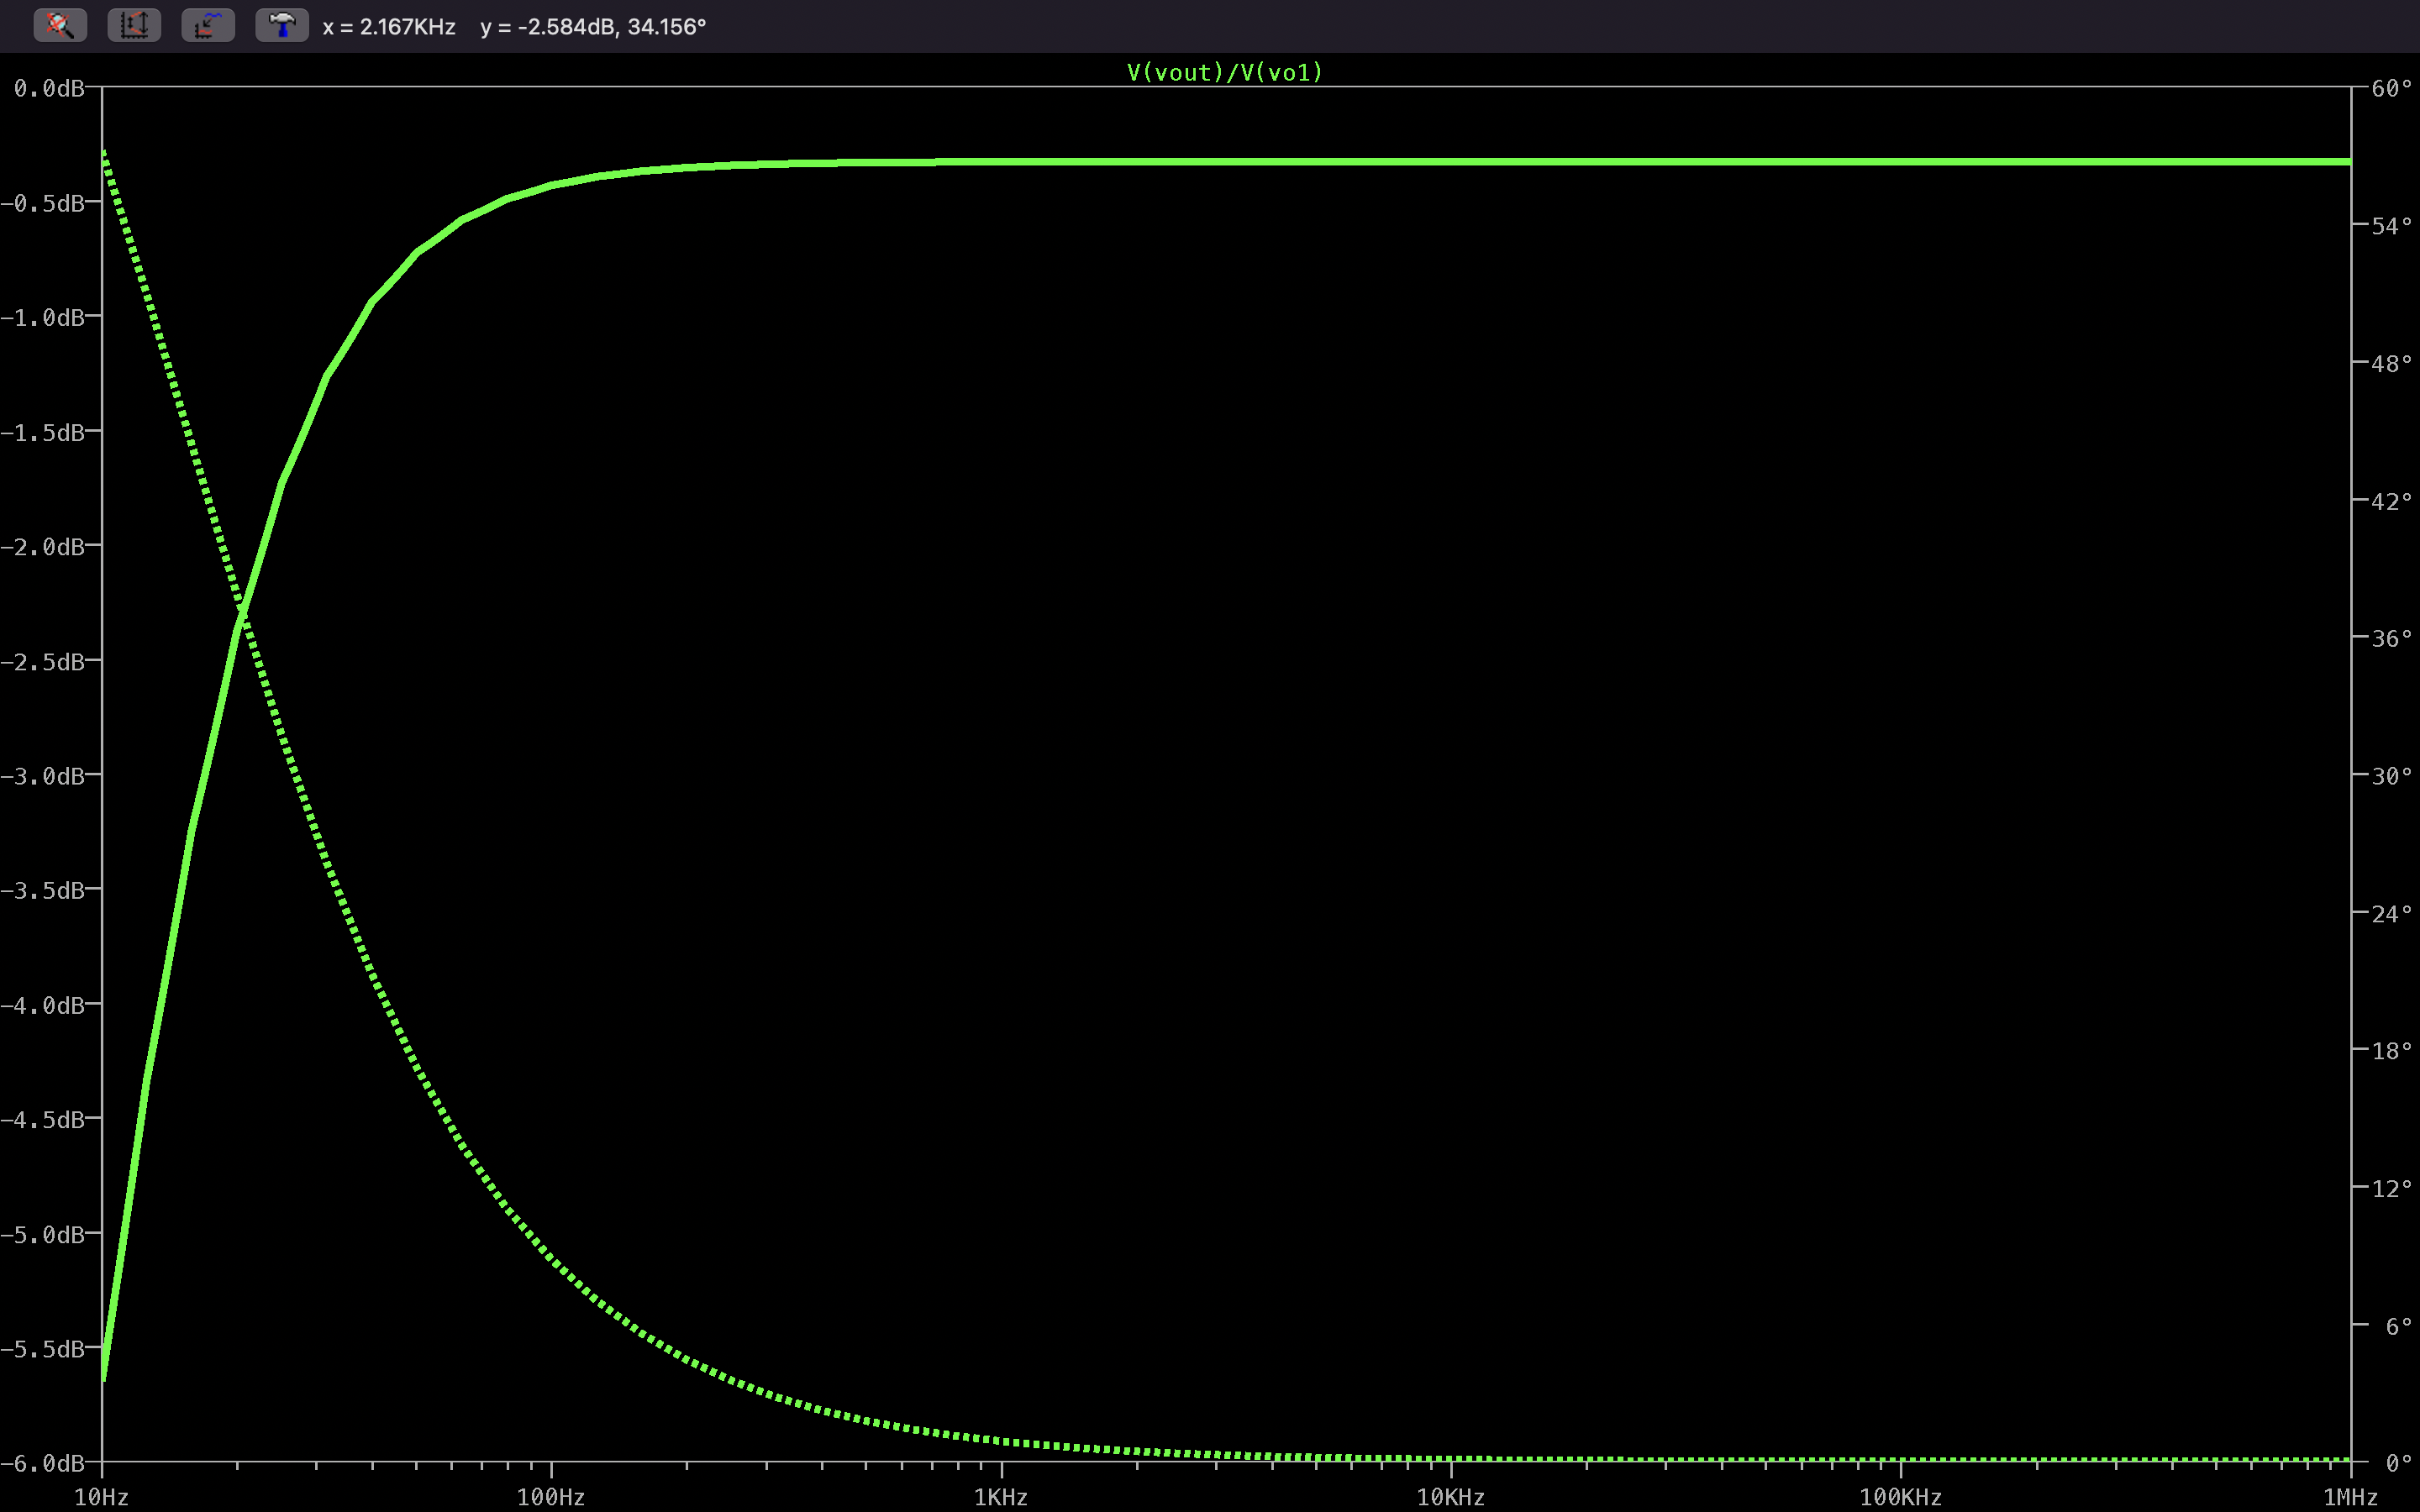
\includegraphics[width=0.9\textwidth]{4.3-2.png} % second figure itself
        					\caption{Representação gráfic  a do ganho A$_{2L}$ em função da frequência de entrada. A$_{2L}$=-0.62329 dB, para 50 kHz}
    						\end{minipage}
				\end{figure}

				\begin{figure}[H]
    					\centering
    					\begin{minipage}{0.45\textwidth}
        					\centering
        					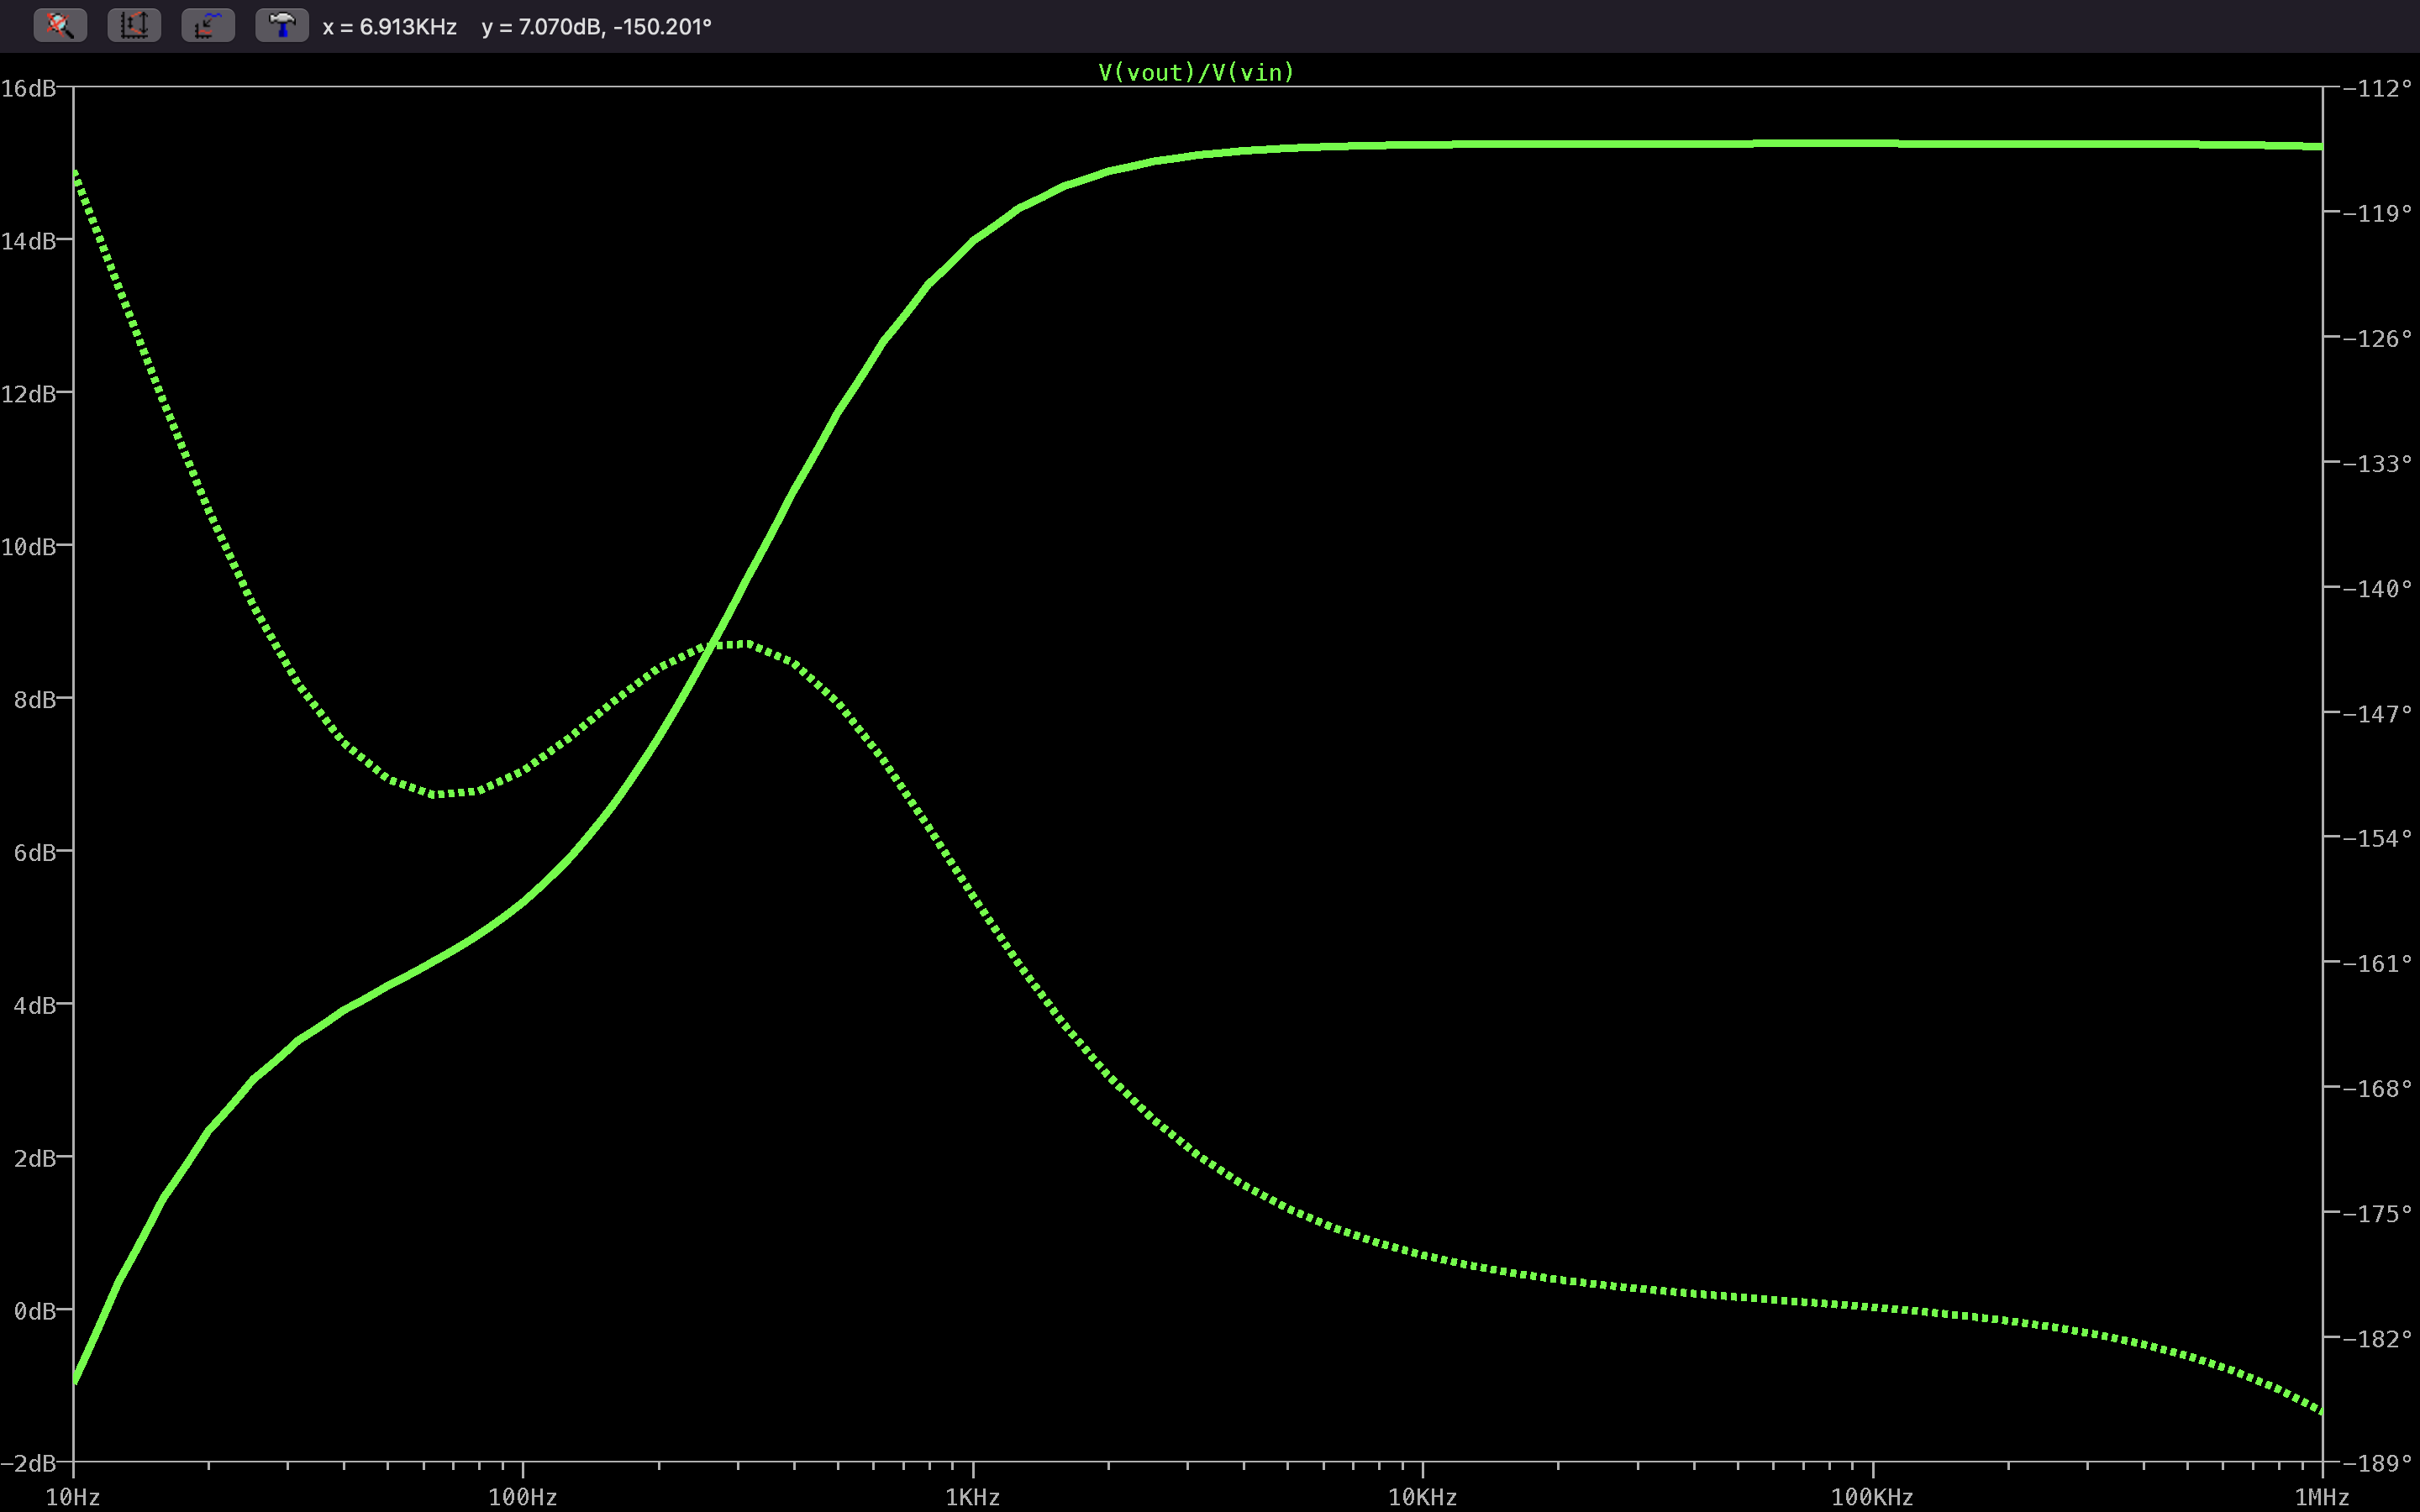
\includegraphics[width=0.9\textwidth]{4.3-3.png} % first figure itself
        					\caption{Representação gráfic  a do ganho A$^´$$_{v}$ em função da frequência de entrada. A$^´$$_{v}$=15.178 dB, para 50 kHz}
    					\end{minipage}\hfill
    					\begin{minipage}{0.45\textwidth}
        					\centering
        					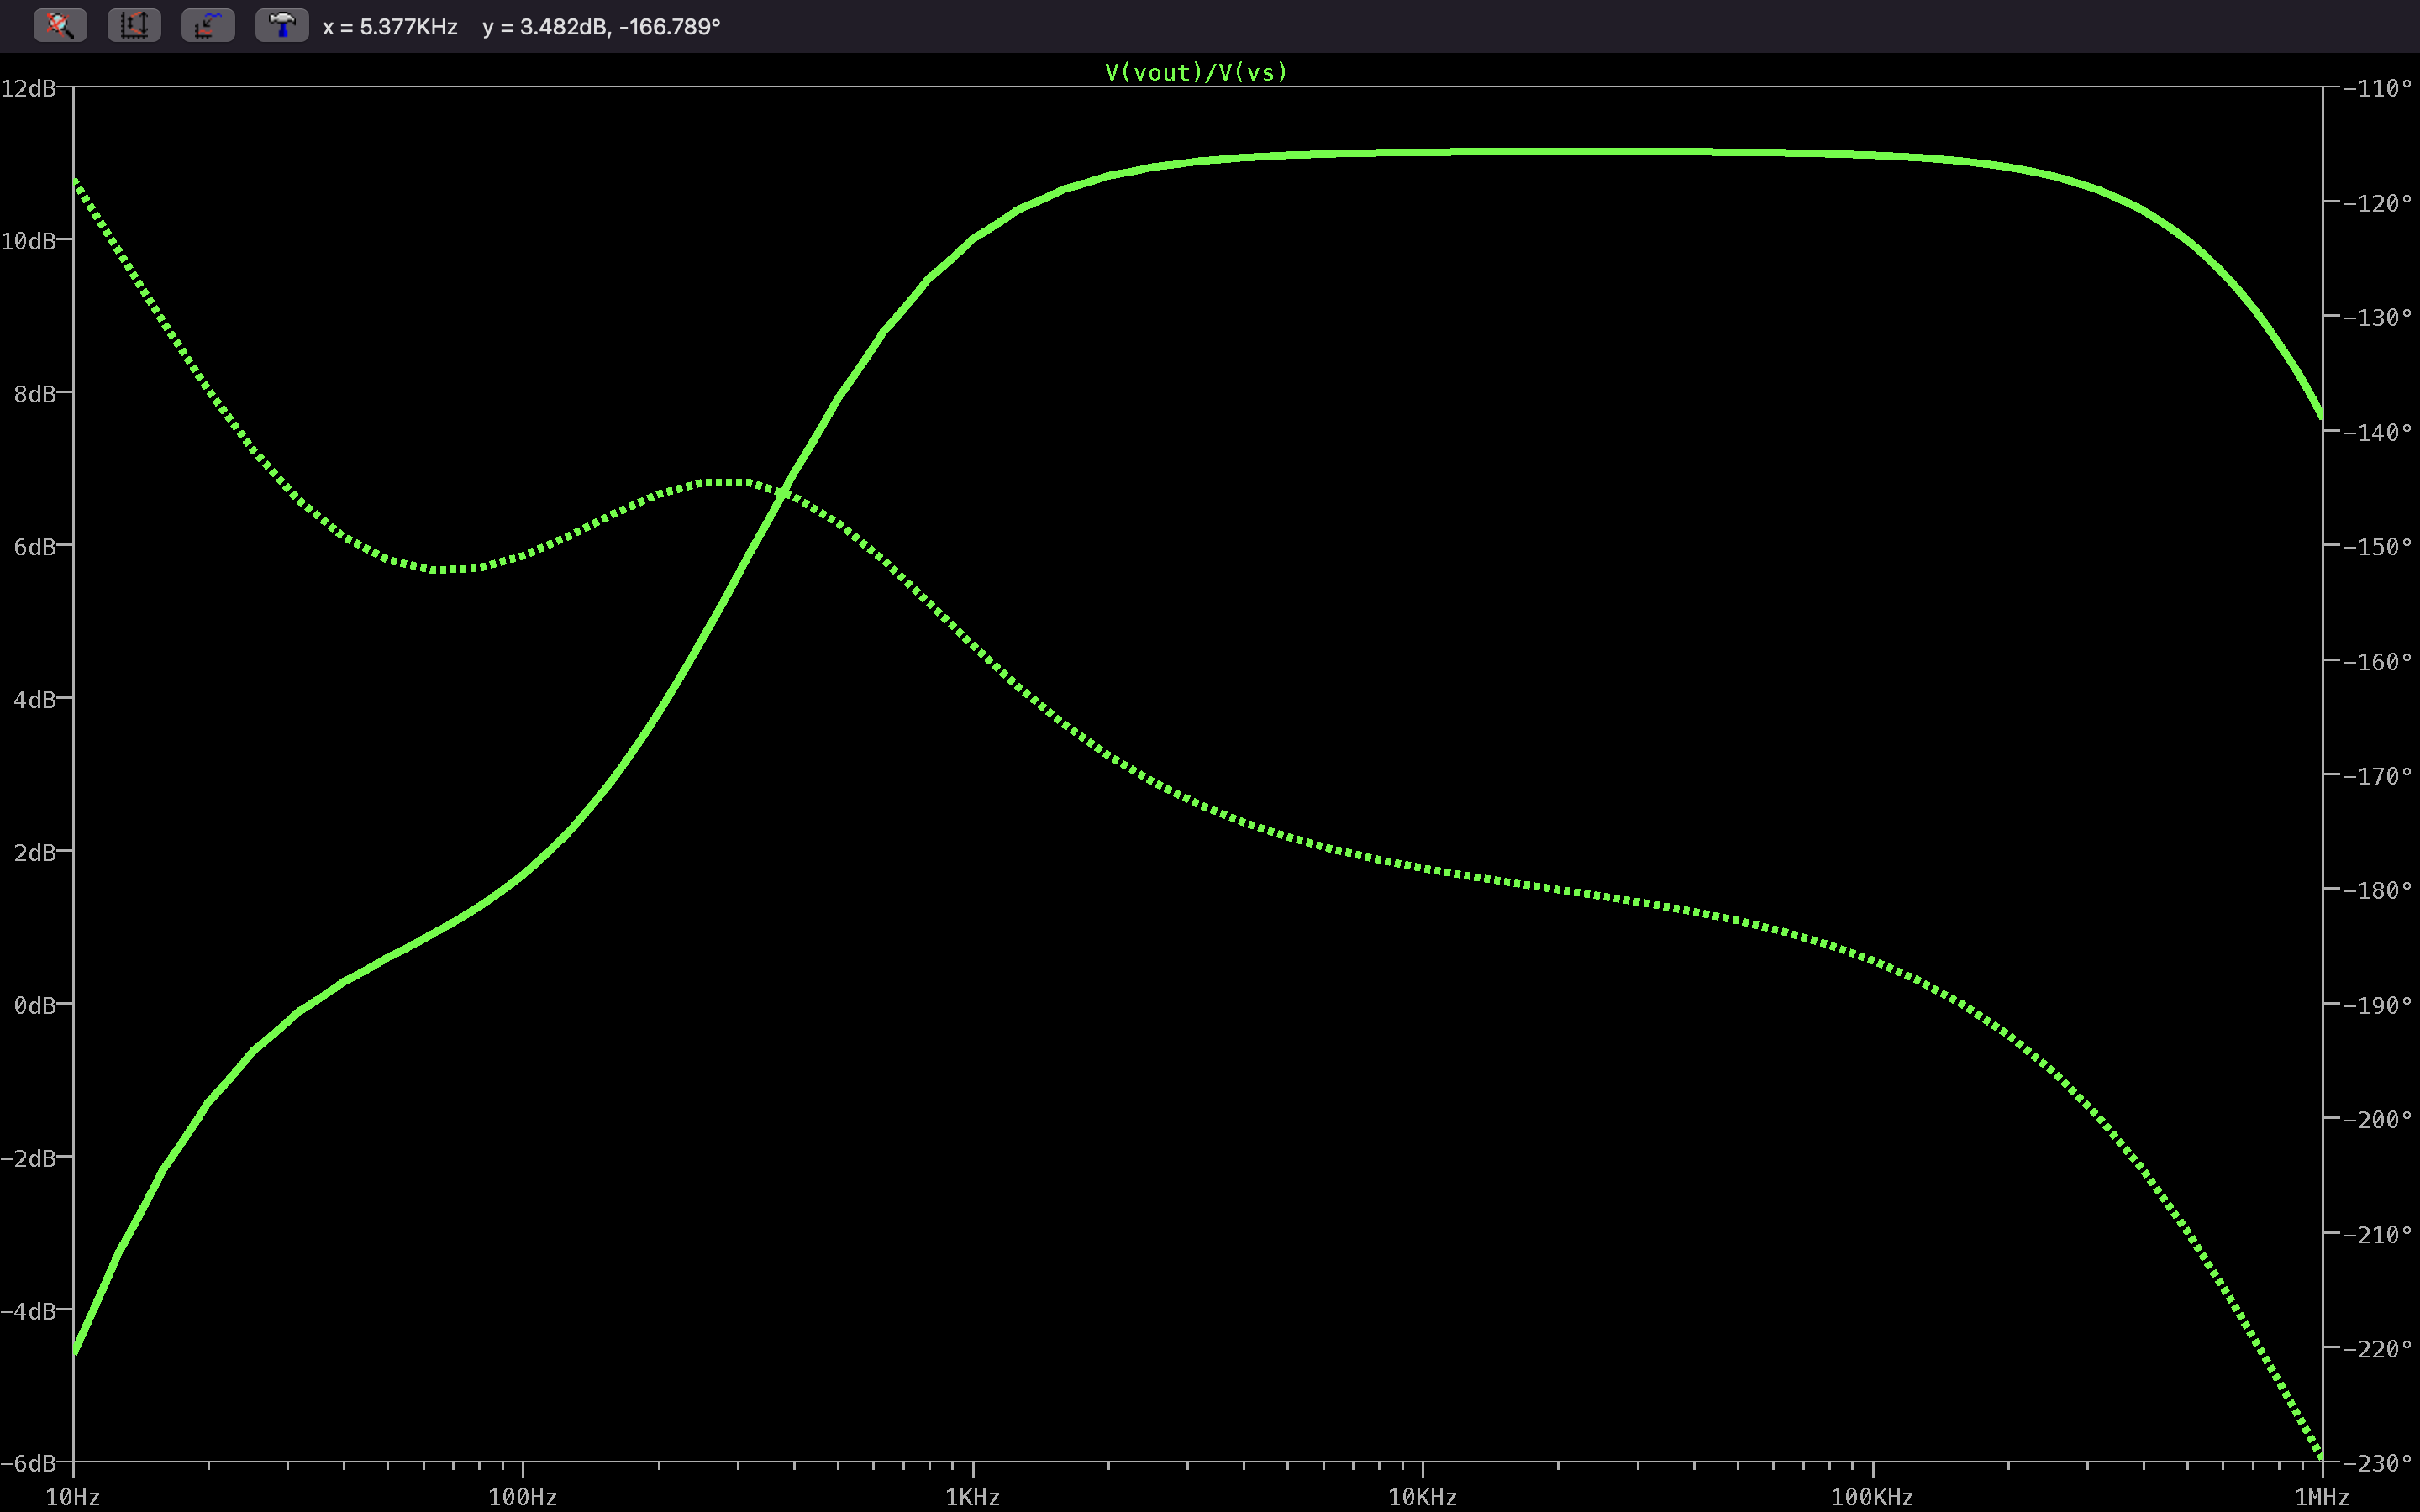
\includegraphics[width=0.9\textwidth]{4.3-4.png} % second figure itself
        					\caption{Representação gráfic  a do ganho A$_{v}$ em função da frequência de entrada. A$_{v}$=10.856 dB, para 50 kHz}
    						\end{minipage}
				\end{figure}


			\subsection{Questão 4.4}
				\begin{figure}[H]
  					\centering
  					\captionsetup{justification=centering}
  					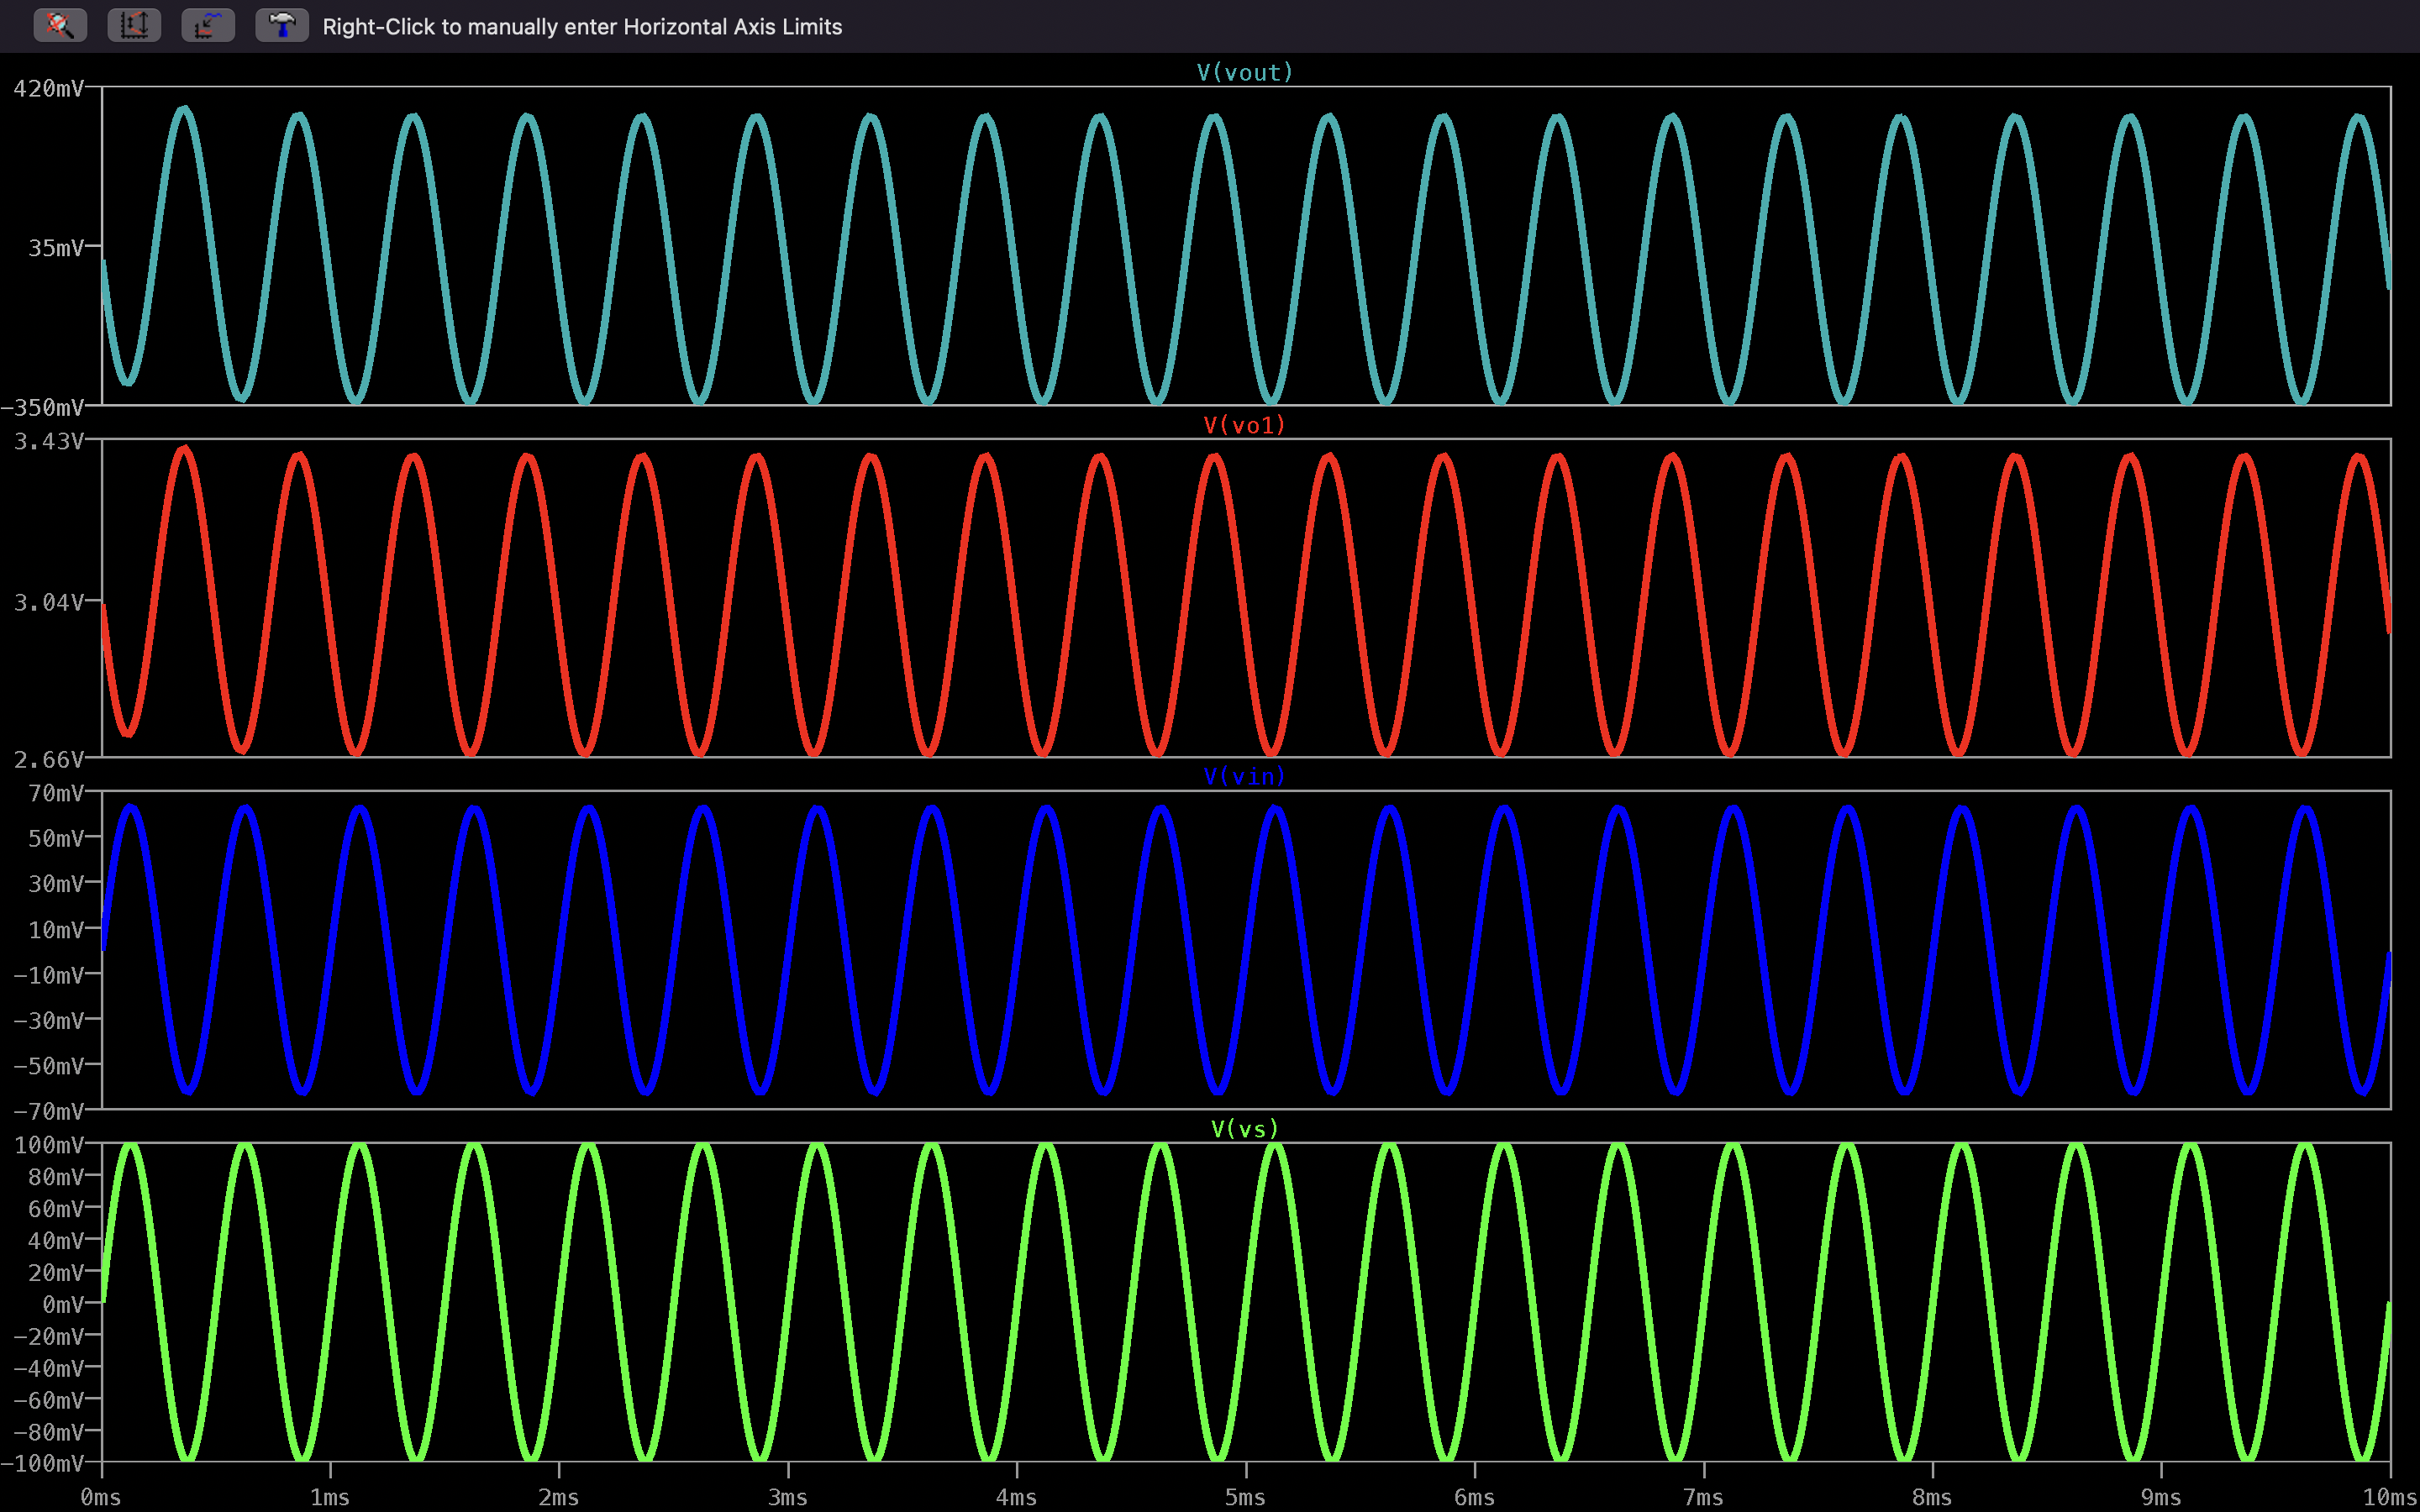
\includegraphics[scale=0.2\textscale]  {4.4.png}
					\caption{V$_{out}$, V$_{o1}$, V$_{in}$ e V$_S$ respectivamente a ciano, laranja, azul e verde. De notar a aproximação entre os valores de V$_{out}$ e V$_{o1}$, resultantes de um ganho aproximadamente unitário no segundo andar do amplificador}
				\end{figure}


			\subsection{Questão 4.5}
				\begin{figure}[H]
  					\centering
  					\captionsetup{justification=centering}
  					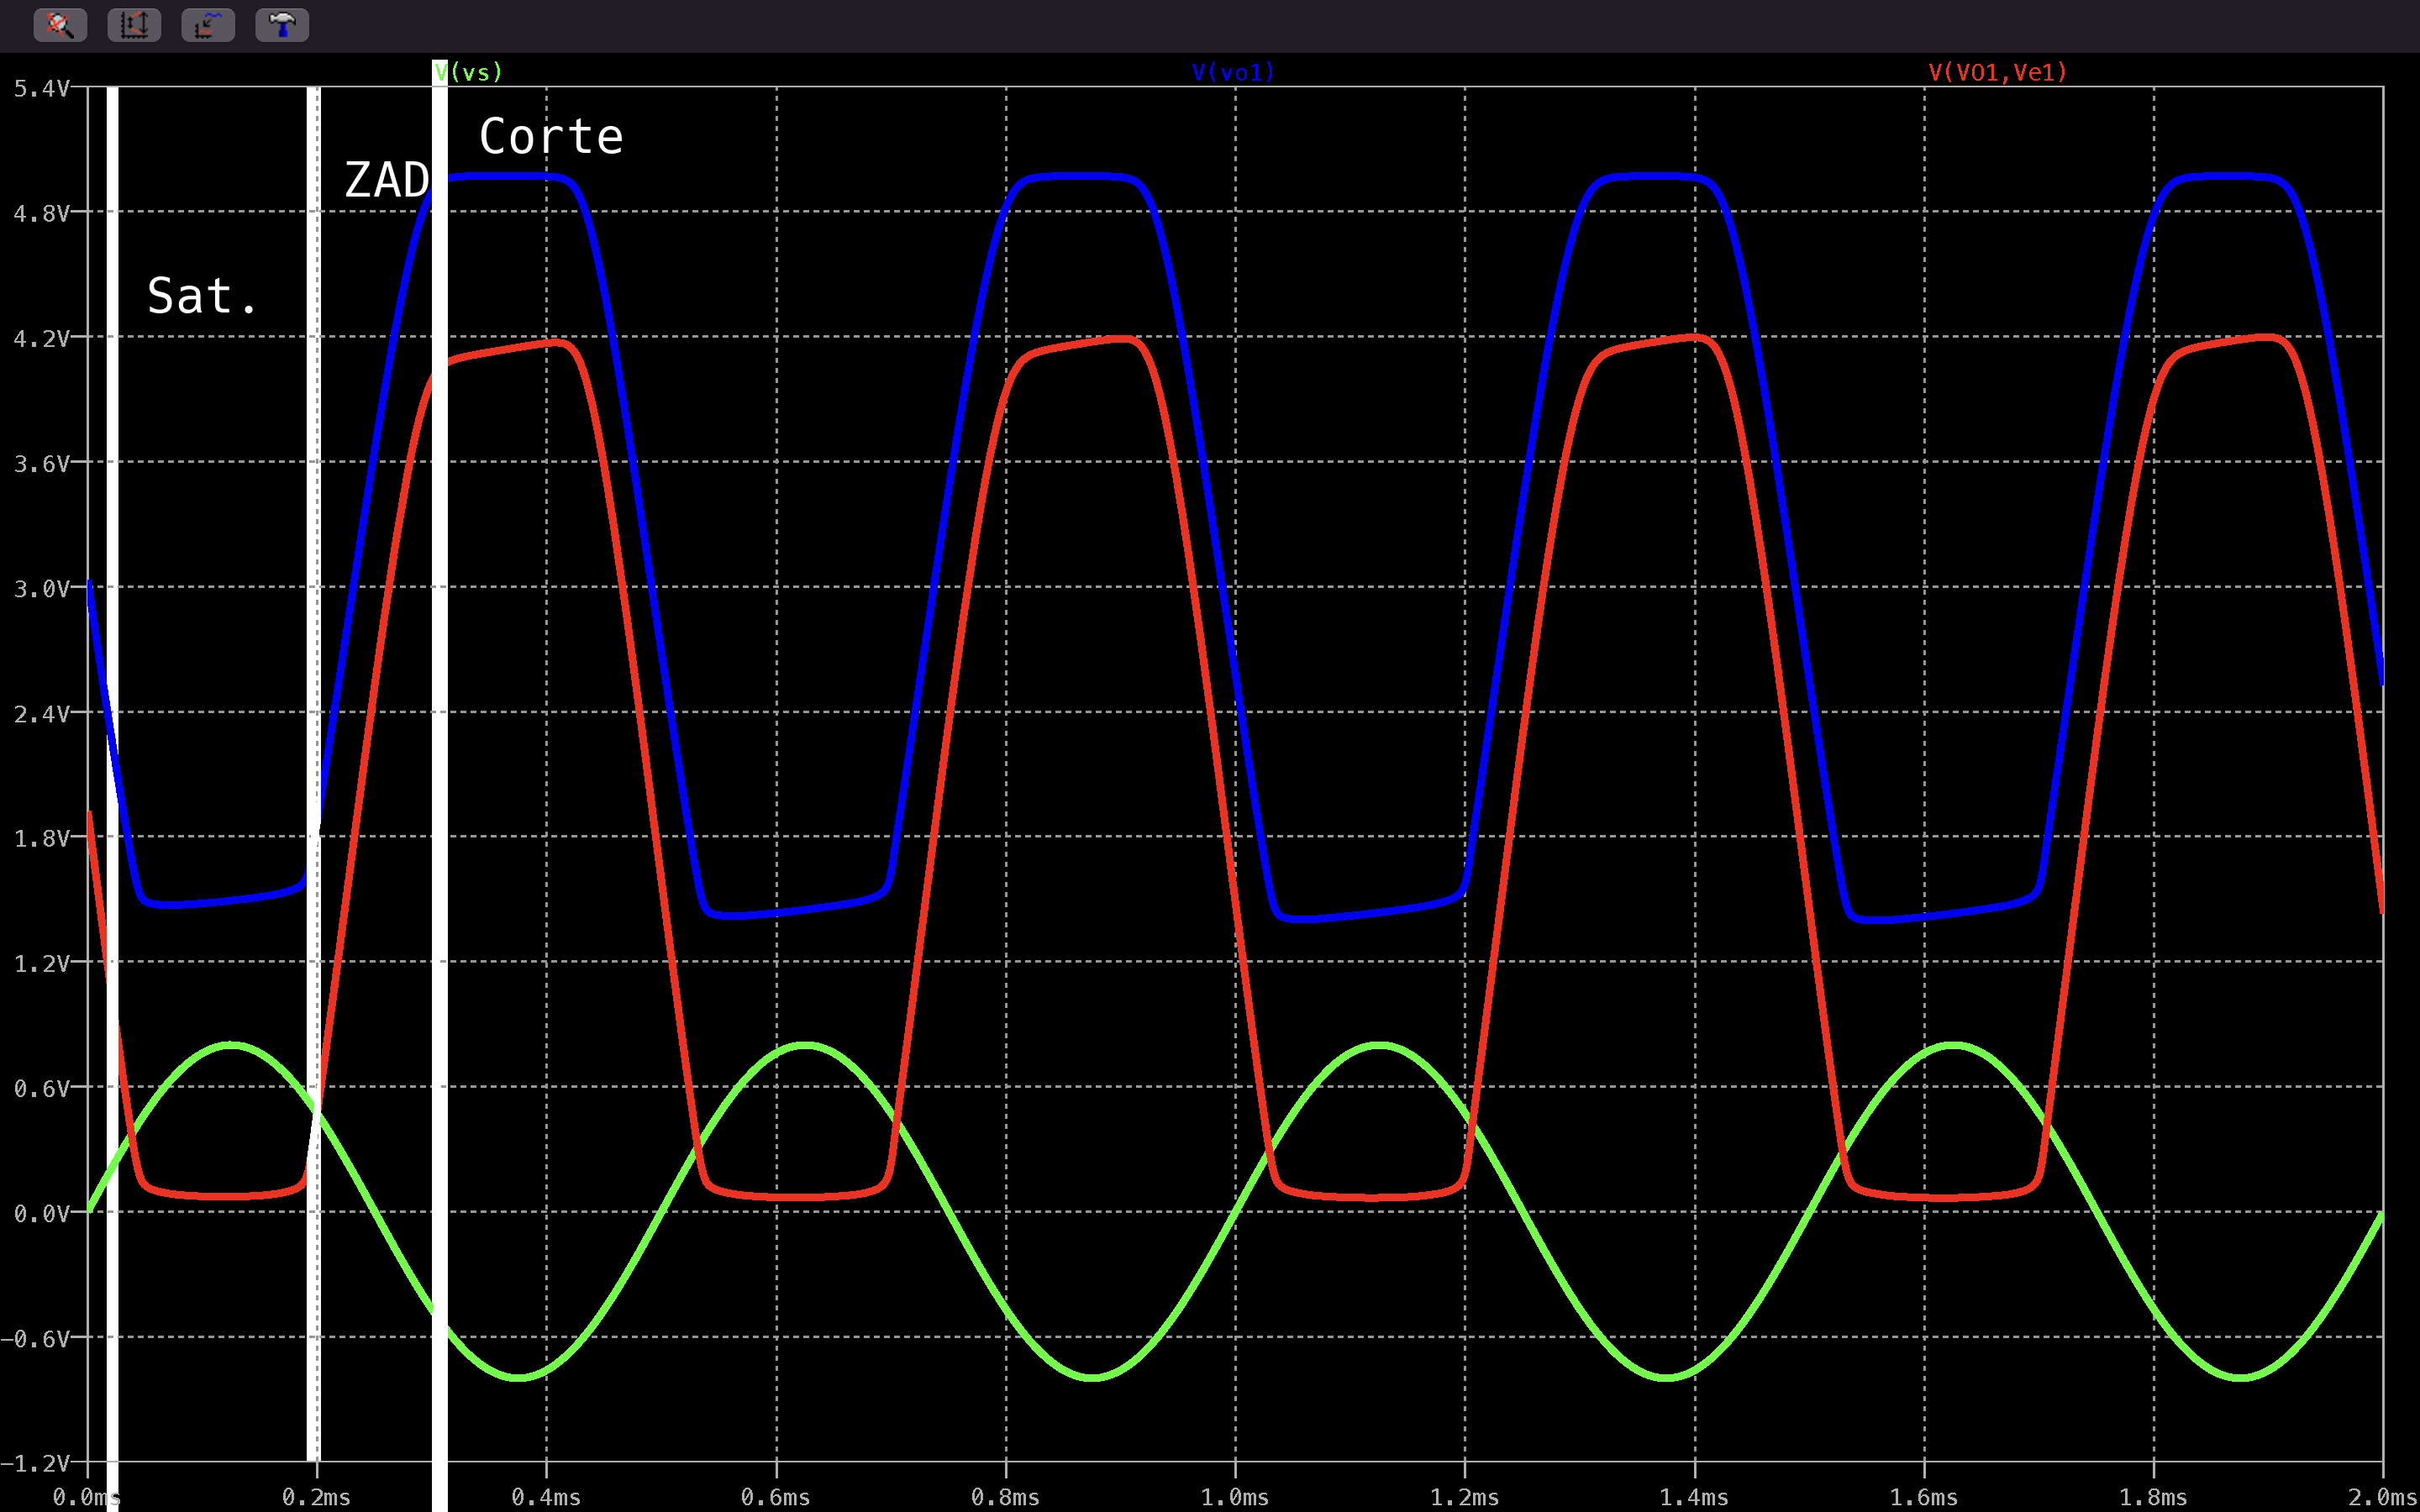
\includegraphics[scale=0.1\textscale]  {4.5.png}
					\caption{Representação gráfica dos diferentes regimes de operação do transístor Q1. Em resumo a identificação das zonas de trabalho pode ser feita pelo seguinte método: Na zona de corte a corrente que passa pelo transístor é nula, sendo V$_{o1}$ = V$_{Vcc}$, aproximadamente 5 V. A zona de saturação é atingida quando a diferença de potencial entre o coletor e o emissor é igual à tensão de saturação específicada pelo fabricante (0.6V).}
					

				\end{figure}


			\subsection{Questão 4.6}
				\begin{figure}[H]
                                          \centering
                                          \captionsetup{justification=centering}
                                          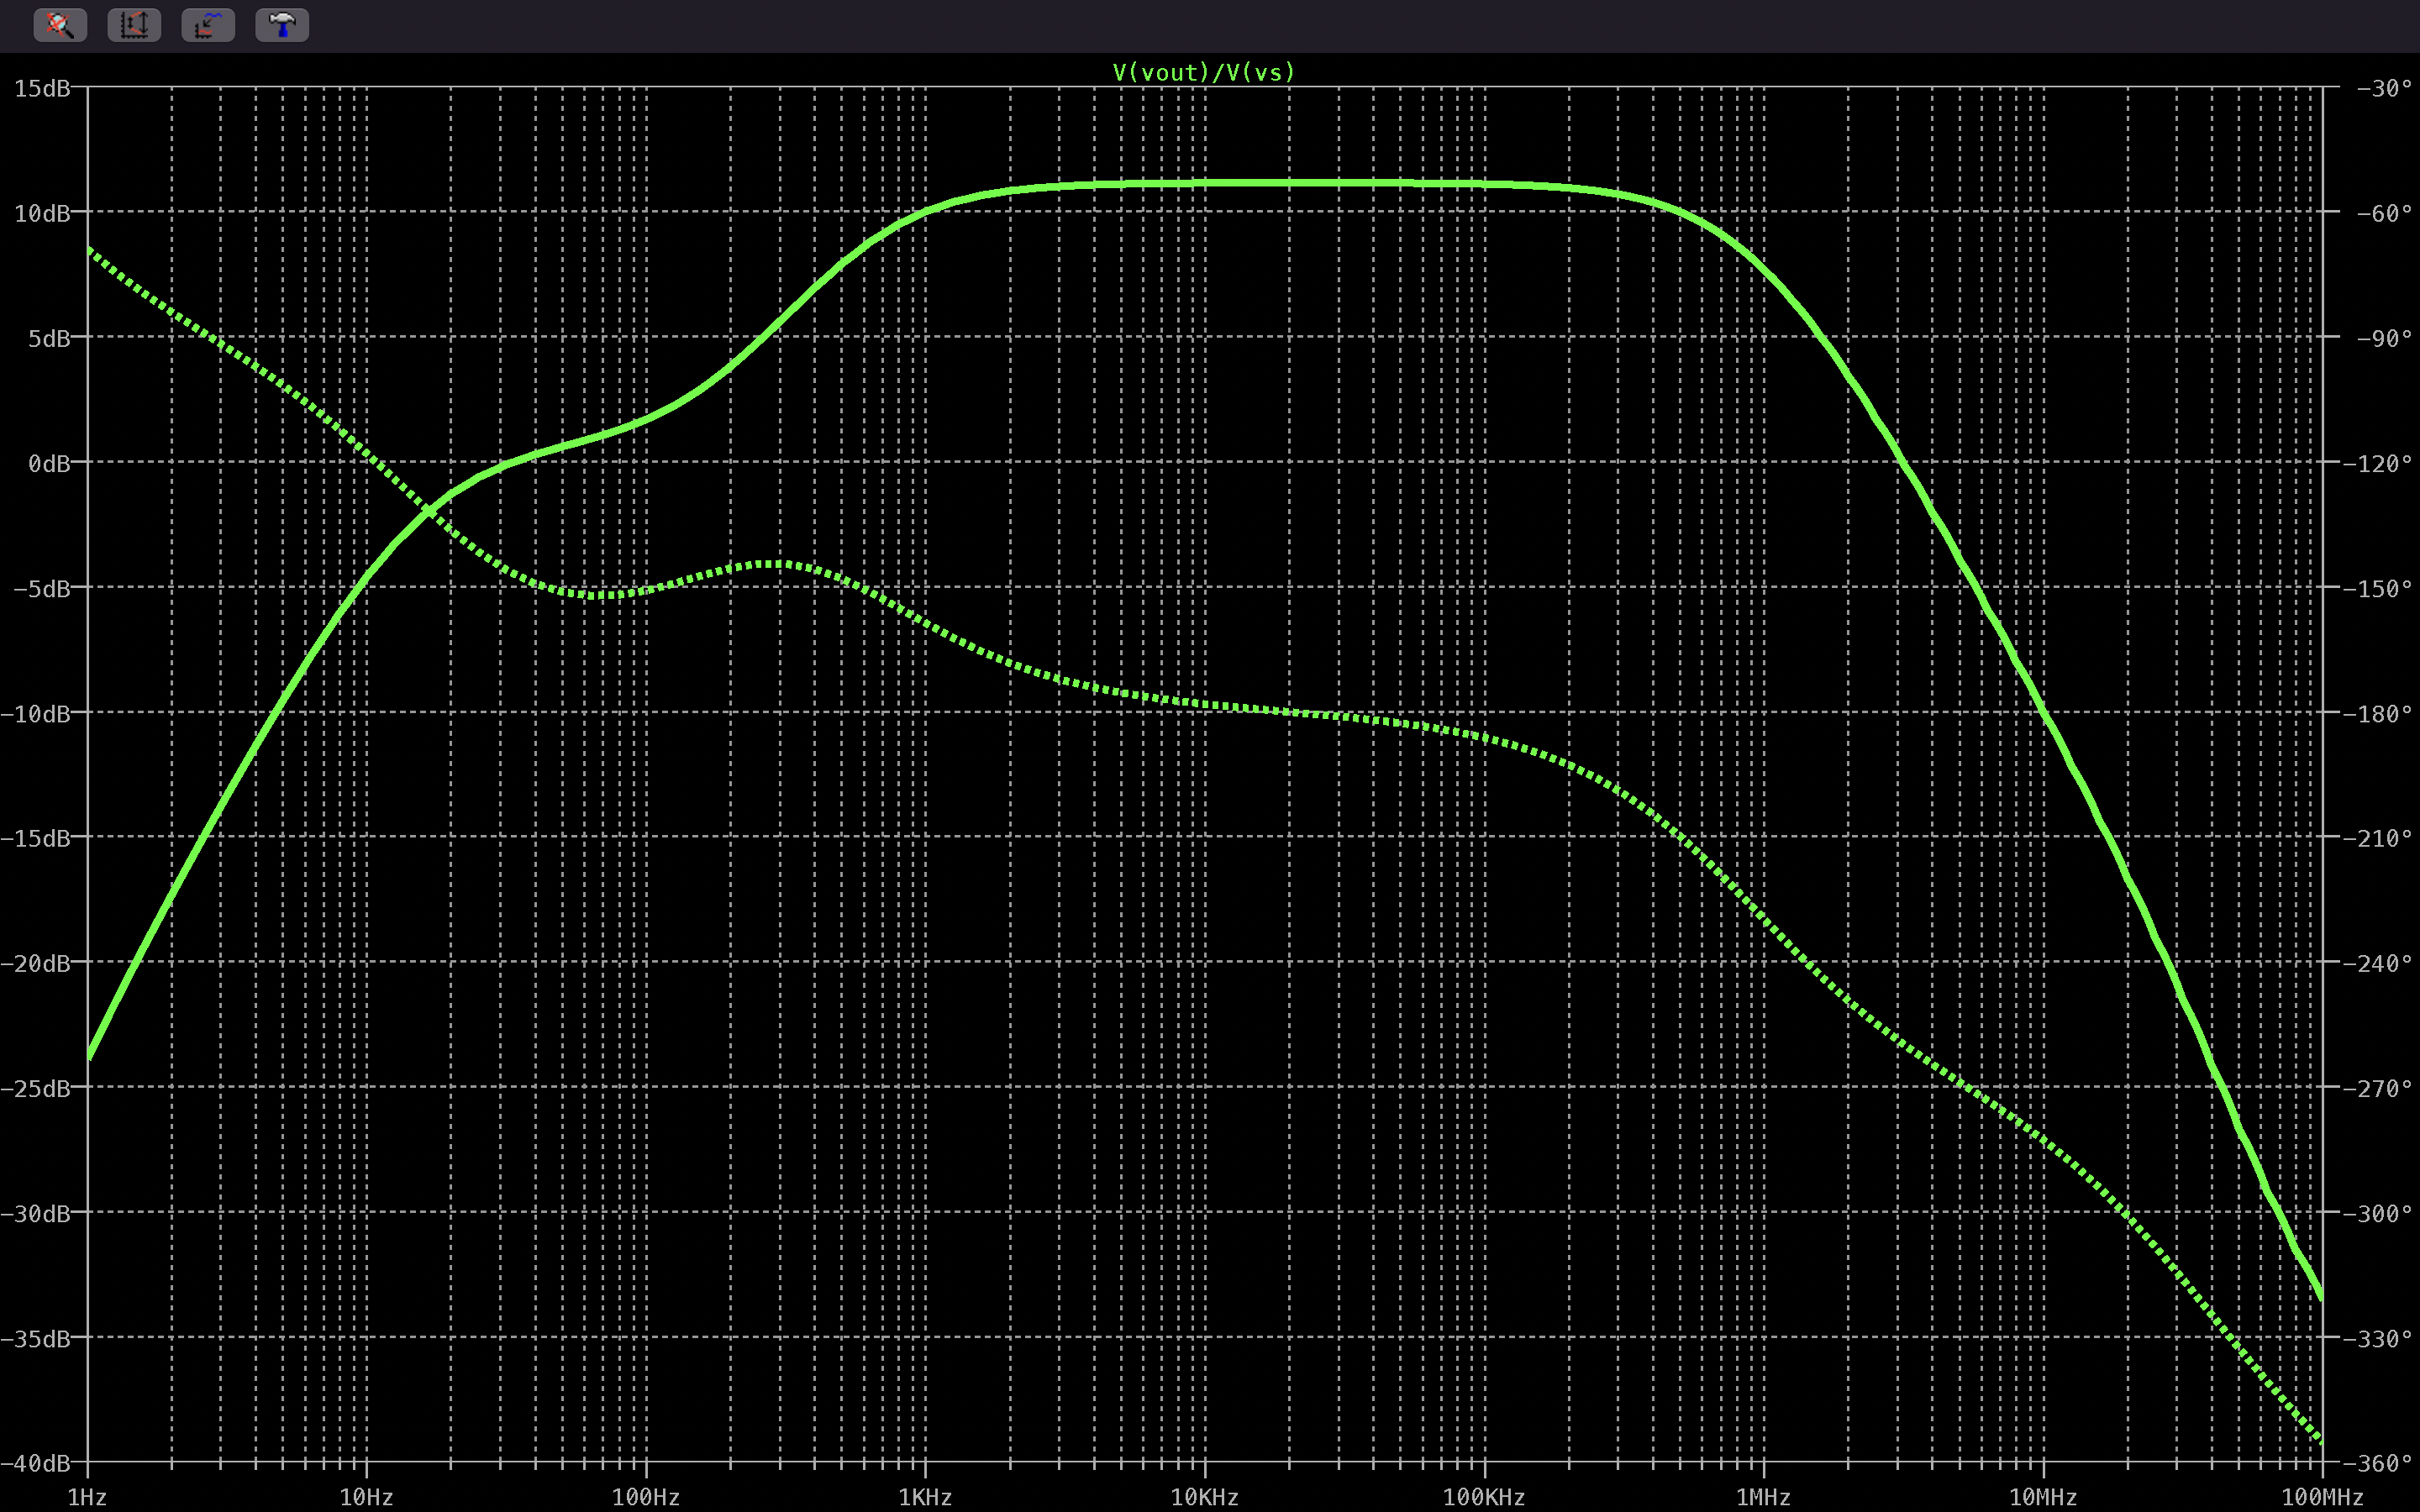
\includegraphics[scale=0.3\textscale]  {4.6.png}
                                          \caption{Representação gráfica da resposta em frequência do amplificador. Com base nesta é possível determinar a largura de banda baseado nos pontos correspondentes a uma queda de 3 dB do ganho da frequência central (de controlo- 50 kHz). Assim por observação do gráfico identifica-se o limite inferior cerca de 500 Hz e o limite superior cerca de 919 kHz, obtendo um valor de largura de banda de 918.5 KHz. É importante notar que o limite superior deste factor é determinado pelos condensadores C1 e C2 apenas}
                                  \end{figure}
		\clearpage
		\section{Questão 5}
			\subsection{Montagem e Questão 5.2}
					\begin{minipage}{0.45\textwidth}
					\begin{table}[H]
					\begin{tabular}{|l|c|}
						\hline
						\textbf{VCC}  &  5 V\\ \hline
						\textbf{VB1} &  1.7137 V\\ \hline
						\textbf{VC1} &  3.011 V\\ \hline
						\textbf{VE1}  &  1.1059 V\\ \hline
						\textbf{VE2} &  2.560 V\\ \hline
						\textbf{VC2} &  4.897 V\\ \hline
					\end{tabular}

				\end{table}
				\end{minipage}
				 \hfill
                                  \begin{minipage}[]{0.45\textwidth}
                                            \captionsetup{justification=centering}
                                            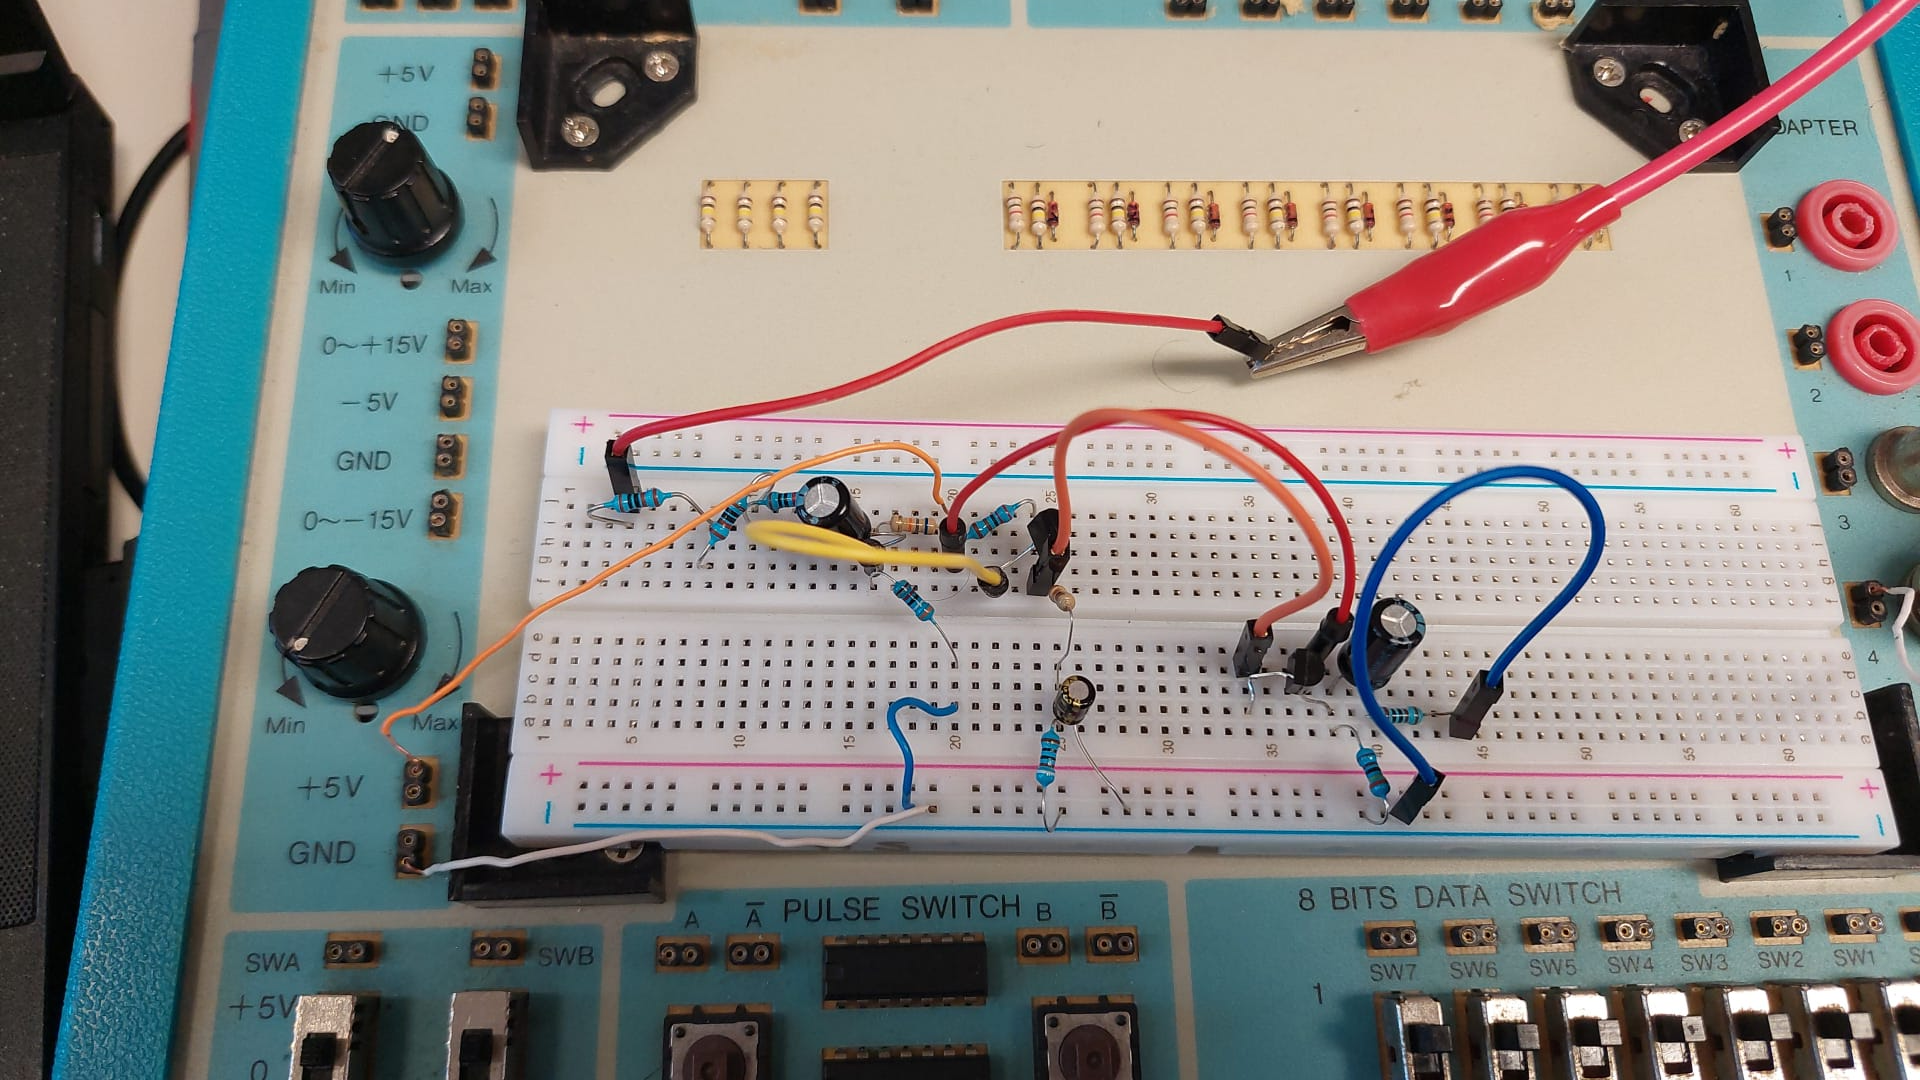
\includegraphics[scale=0.1\textscale]{montagem.png}
                                        \captionof{figure}{Montagem do amplificado r de dois andares, com transístores BJT, BC547B.}

                                  \end{minipage}
				\\ É possível então determinar pela Lei de Ohm:\\
				\begin{equation}
					I_{C1}=\frac{V_{CC}-V{C1}}{R_C}= 0.9041 mA
				\end{equation}
				\begin{equation}
					I_{C2}=\frac{V_{E2}-V{GND}}{R_{E3}}=1.0667 mA
				\end{equation}



			\clearpage
			\subsection{Questão 5.4}
					\begin{figure}[H]
    					\centering
    					\begin{minipage}[t]{0.45\textwidth}
        					\centering
        					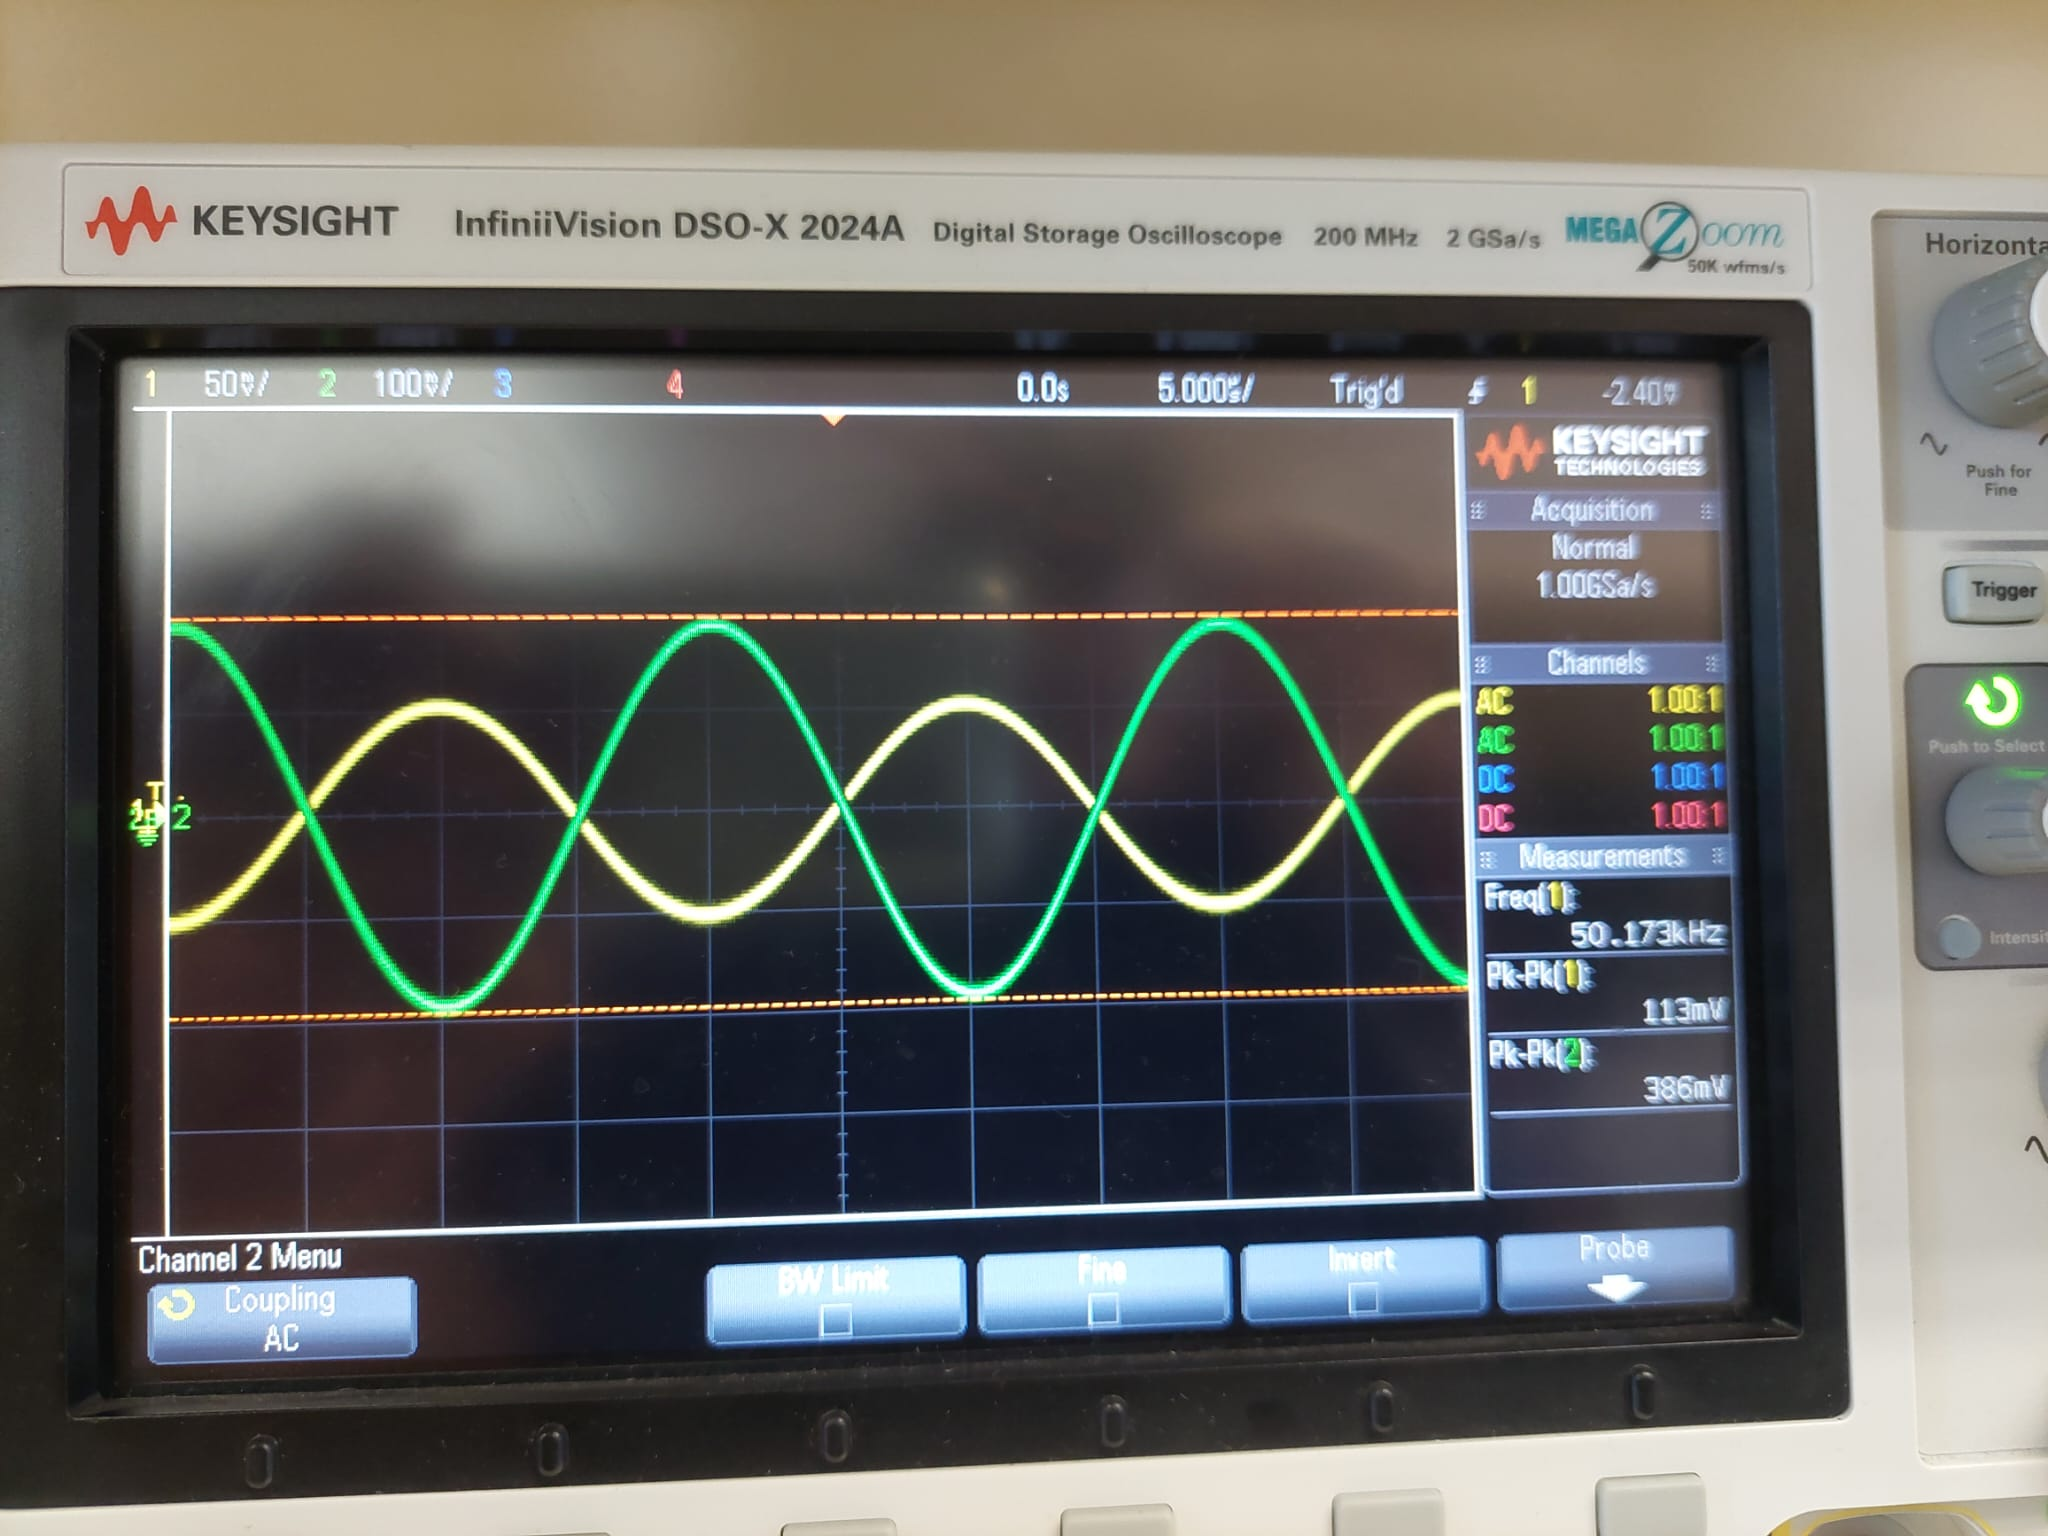
\includegraphics[width=0.9\textwidth]{5.4-1.jpeg} % first figure itself
        					\caption{Representação gráfica de V$_{out}$ para 110 mV de tensão de entrada (V$_S$, 50 kHz). V$_{out}$ pico a pico = 386 mV}
    					\end{minipage}\hfill
    					\begin{minipage}[t]{0.45\textwidth}
        					\centering
        					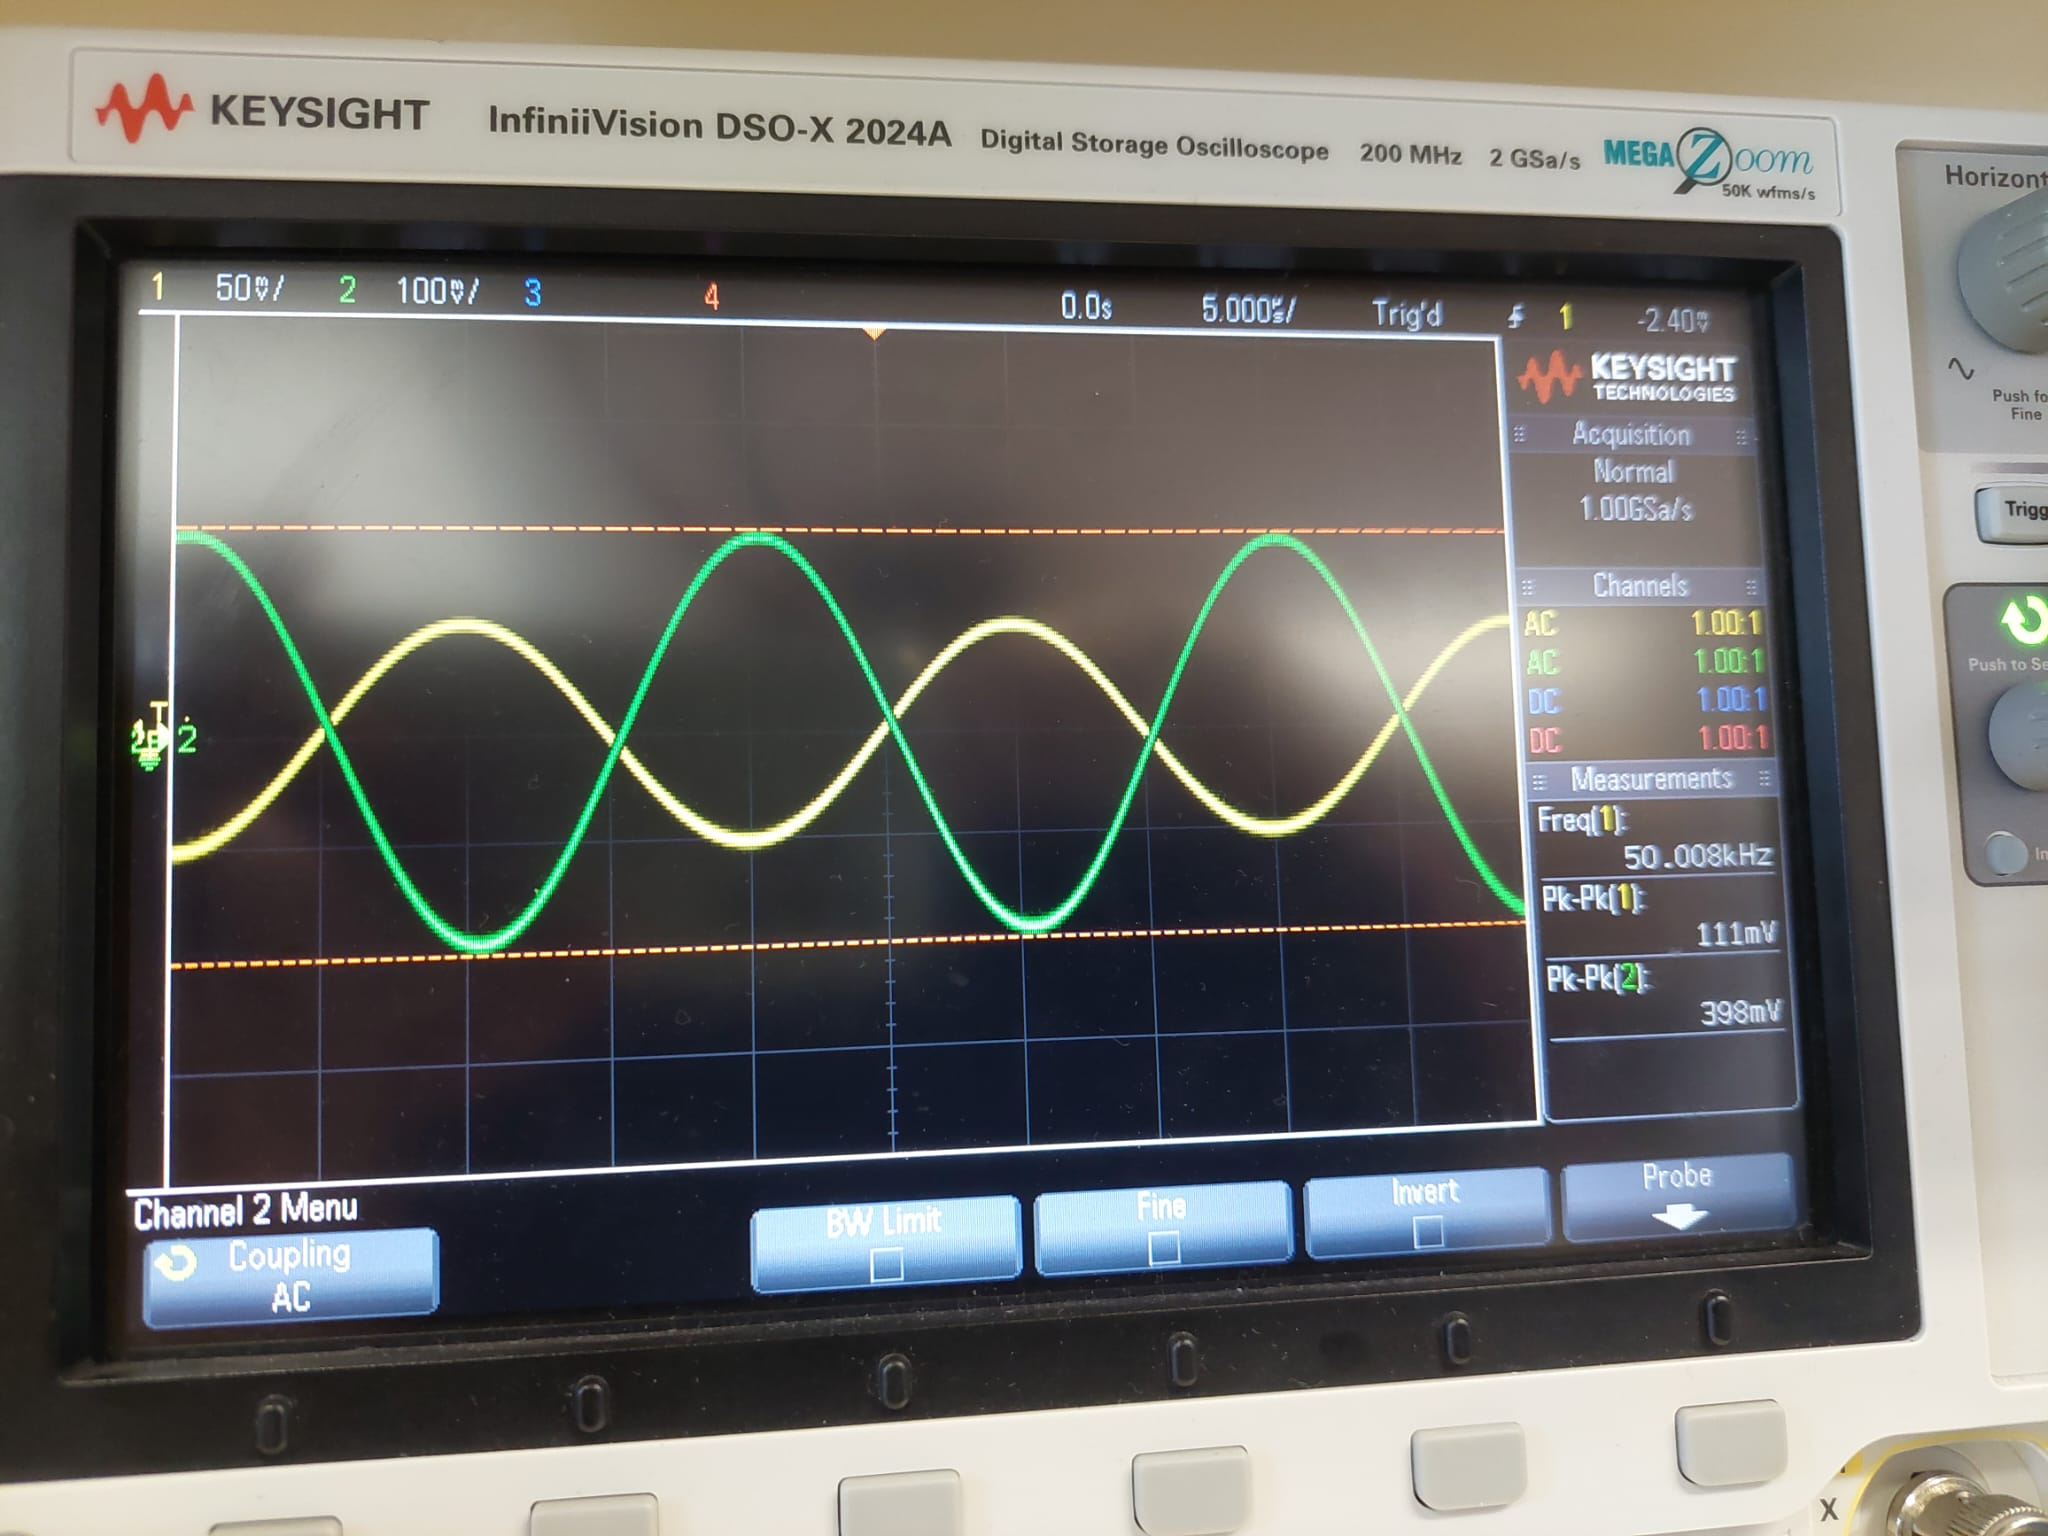
\includegraphics[width=0.9\textwidth]{5.4-2.jpeg} % second figure itself
        					\caption{Representação gráfica de V$_{o1}$ para 110 mV de tensão de entrada (V$_S$, 50 kHz). V$_{o1}$ pico a pico = 398 mV}
    						\end{minipage}
				\end{figure}
				
				\begin{figure}[H]
  					\centering
  					\captionsetup{justification=centering}
  					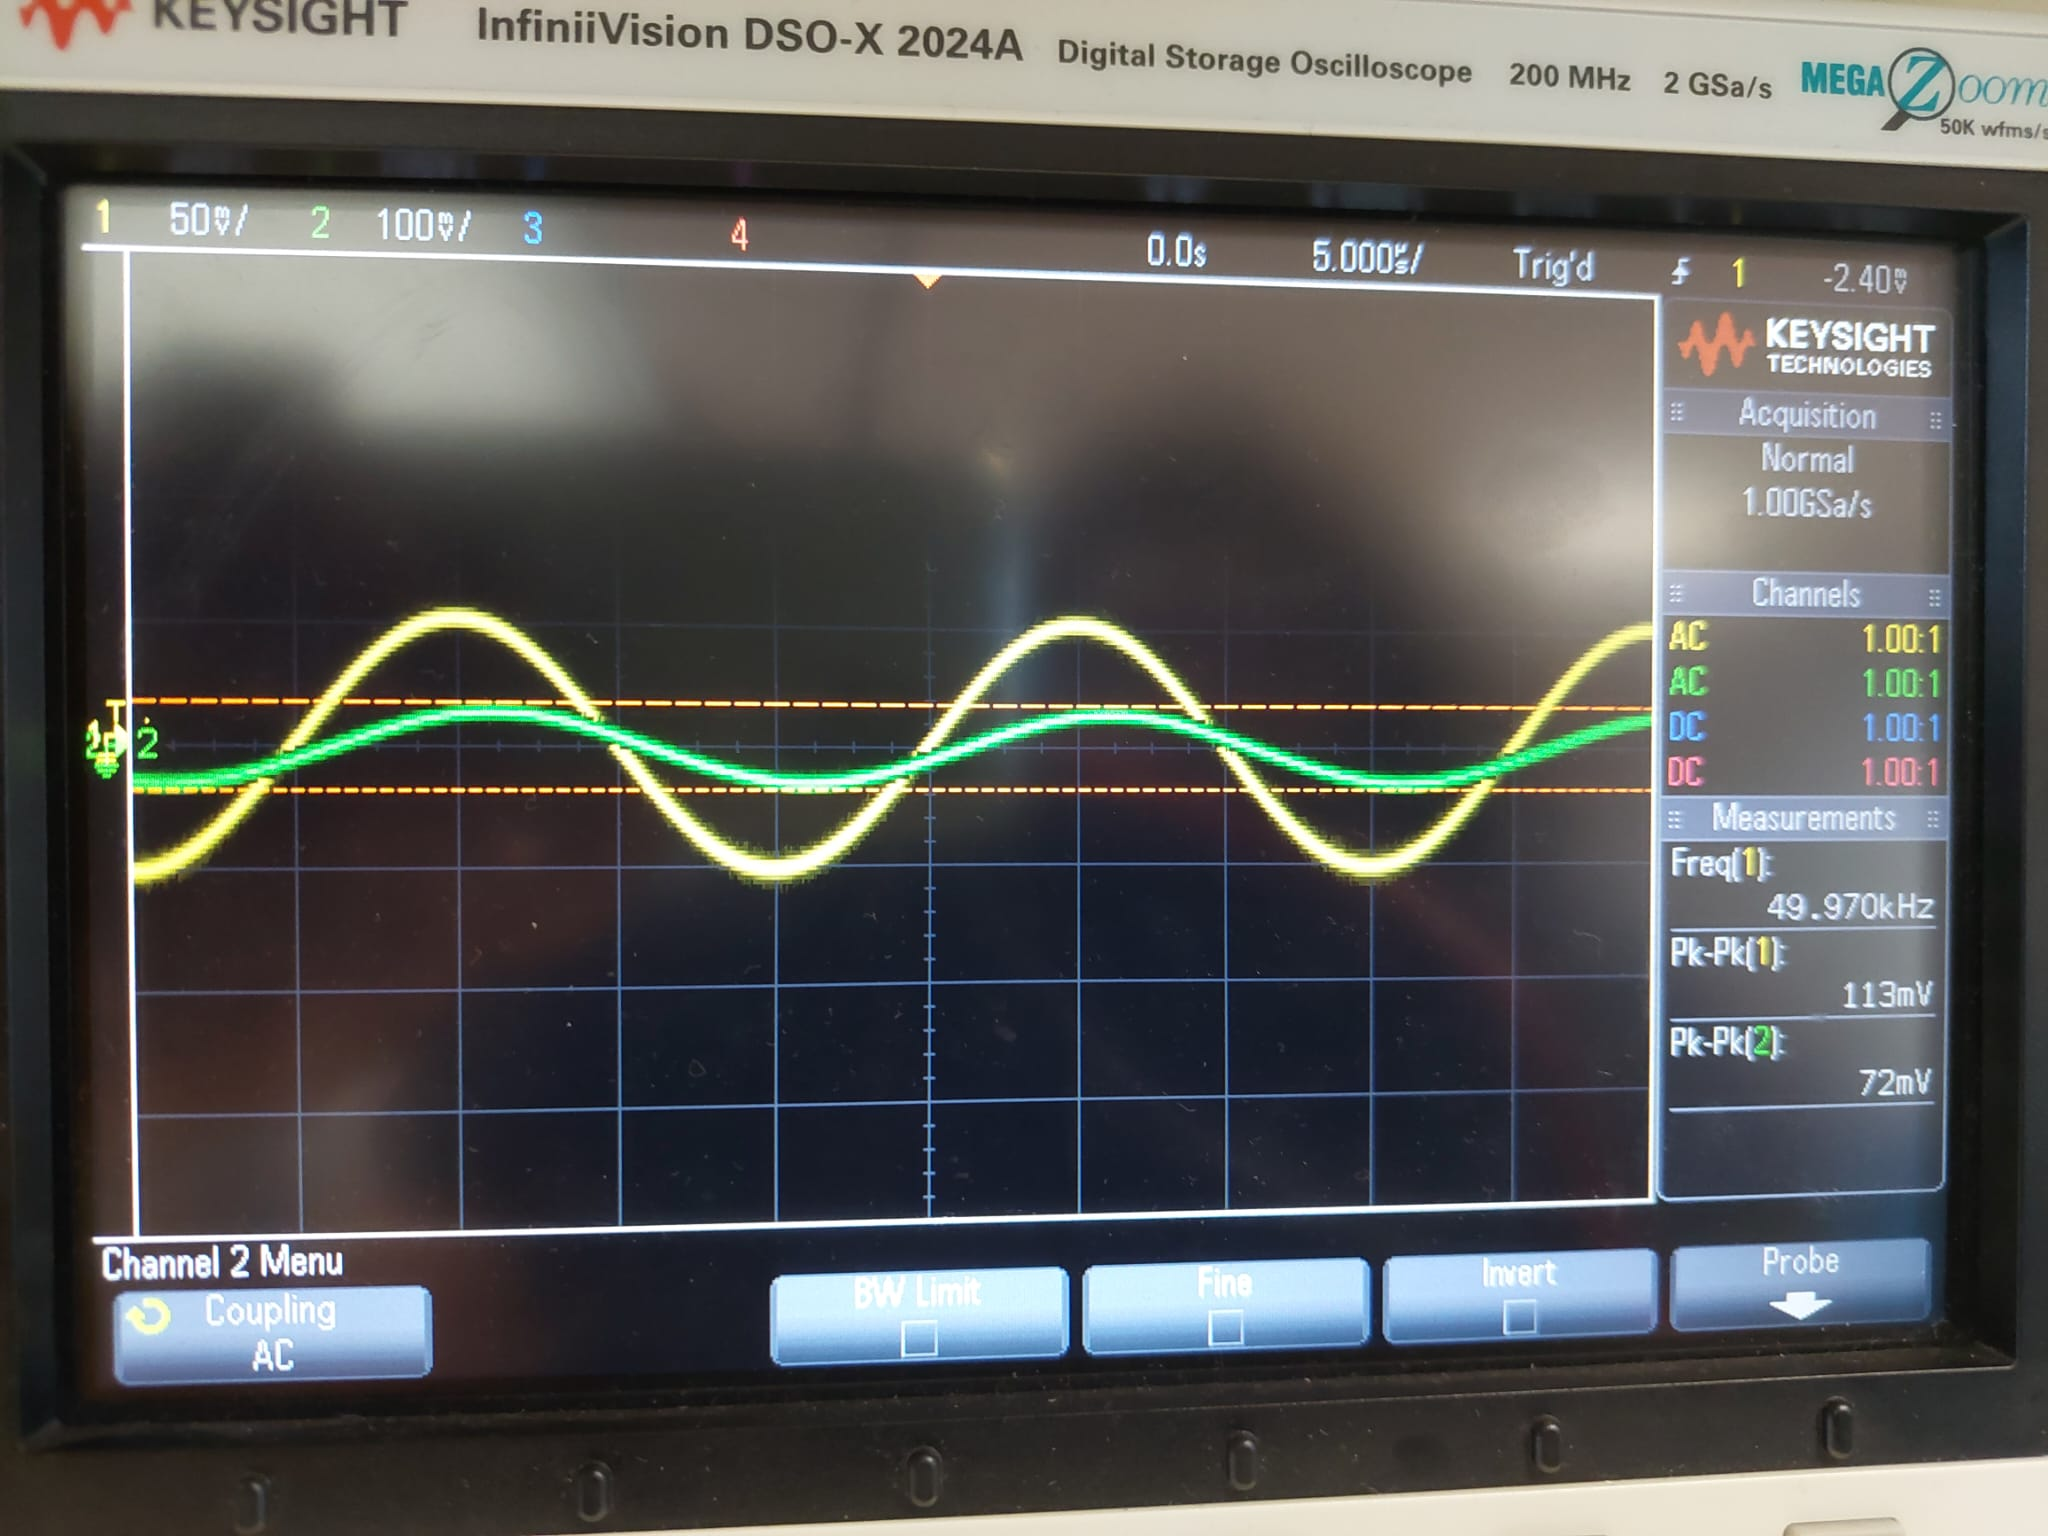
\includegraphics[scale=0.1\textscale]  {5.4-3.jpeg}
					\caption{Representação gráfica de V $_{in}$ para 110 mV de tensão de entrada (V$_S$, 50 kHz). V$_{in}$ pico a pico = 72 mV}
				\end{figure}



			
			\subsection{Questão 5.5}
				Utilizando os valores obtidos na Questão 5.4:
				\begin{center}
					\begin{equation}
						A_{1L}=20 \times log \frac{V_{o1}}{V_{in}} = 14.85 dB
					\end{equation}
					\begin{equation}
						A_{2L}=20 \times log \frac{V_{out}}{V_{o1}} = - 0.266 dB
                                        \end{equation}
					\begin{equation}
						A^{´}_{v}=20 \times log \frac{V_{out}}{V_{in}} = 14.585 dB
                                        \end{equation}
					\begin{equation}
						A_{v}=20 \times log \frac{V_{out}}{V_S} = 10.903 dB
                                        \end{equation}
				\end{center}

			\clearpage
			\subsection{Questão 5.6}
					   \begin{figure}[H]
                                          \centering
                                          \captionsetup{justification=centering}
                                          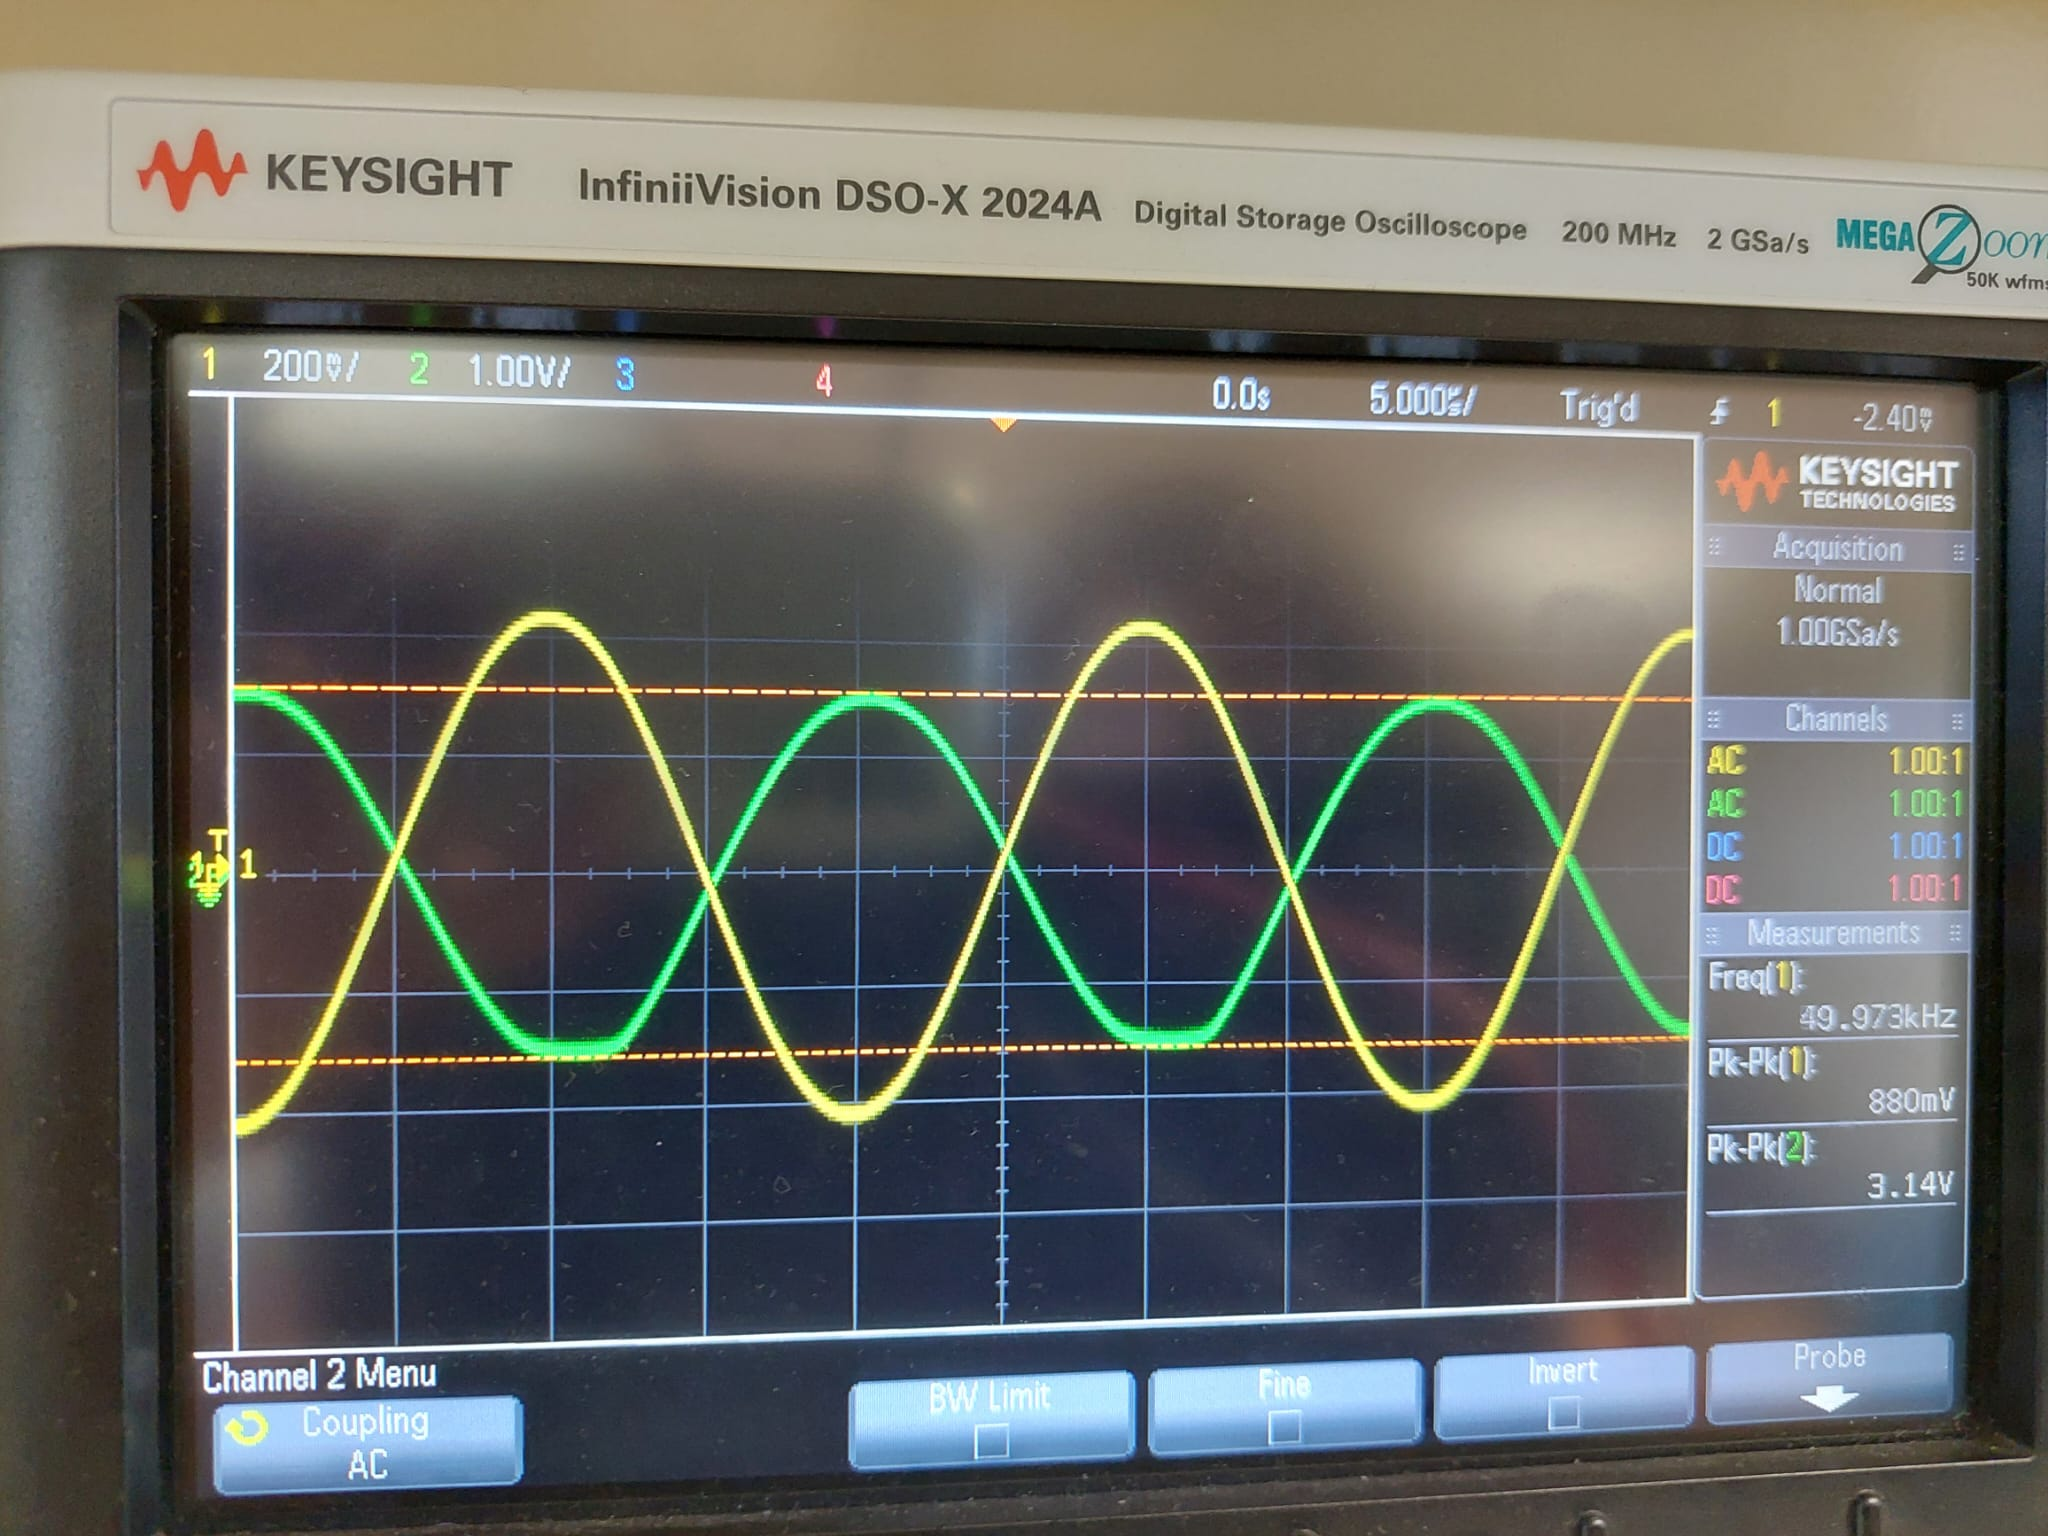
\includegraphics[scale=0.2\textscale]  {5.6.jpeg}
                                          \caption{Representação gráfica de V  $_{o1}$ para 880 mV de tensão de entrada (V$_S$, 50 kHz). De notar a a forma sinusoidal de V$_S$, em oposição à clara sinusoide distorcida representativa de V$_{o1}$.}
                                  \end{figure}
			\subsection{Questão 5.7}
				\begin{table}[H]
                                            \centering
                                            \begin{tabular}{|l|c|}
                                                    \hline
						    \textbf{Tensão de controlo} & 386 mV \\ \hline
                                                    \textbf{Limite}$_{inferior}$  & 502.6 Hz \\ \hline
                                                    \textbf{Limite}$_{superior}$ &  579.4 KHz\\ \hline
                                                    \textbf{Largura de Banda} &  578.9 KHz\\ \hline
                                                    
                                            \end{tabular}

                                    \end{table}
		\clearpage
		\section{Análise de Resultados e Conclusões}
			De forma geral os valores obtidos laboratorialmente encontram-se de acordo com os simulados.\par
			A principal justificação para as discrepâncias entre os valores teóricos e práticos (nomeadamente a diferença entre as larguras de banda obtidas e os ganhos A$_{2L}$ determinados) advêem de três géneses principais.\par
			Em primeiro lugar os métodos de obtenção dos valores teóricos a partir do software \textit{LTSpice} não são os mais precisos, sendo suscetíveis a erros de medição humano.\par
			Em segundo lugar, na prática, o circuito não é perfeito sendo sensível a ruído resultante de maus contactos, nomeadamente entre a breadboard e a estação de trabalho digital.\par
			Por fim é importante não desconsiderar a presença de capacidades parasitas, tanto nos cabo coaxiais como nos transístores. Embora o \textit{LTSpice} faça uma aproximação das capacidades parasitas dos transístores utilizados estas são distintas das reais.
\end{document}







